\documentclass{beamer}
%\usetheme[
%          titlepagelogo=bold50-illinois,% Logo for the first page
%          pageofpages=of,% String used between the current page and the total page count
%          titleline=true,% Show a line below the frame title
%          ]{TorinoTh}

\usetheme{Luebeck}

\usepackage{beamerthemesplit}
\usepackage{graphics}
\usepackage{graphicx}
\usepackage{hyperref}
\usepackage{comment}
\usepackage{ulem}
\usepackage{color} 
\usepackage{xspace}

\newcommand{\bllt}{\item \small}

\newcommand{\doneTask}[1]{\item \small \sout{#1}} 

\newcommand{\MyName}{Vivek~Kale} 

\newcommand{\fixme}[1]{\textcolor{blue}{[FIXME: #1]}}
\newcommand{\revision}[1]{\textcolor{blue}{[FIXME comment : #1]}}

\title{Notes}
\author{\MyName}
\date{\today}

\title[All Notes]{ Notes }
\author[Vivek Kale]{%
  Vivek~Kale\inst{1}}

\institute[University of Illinois at Urbana-Champaign]{
  \inst{1}%
  Department of Computer Science\\
  University of Illinois at Urbana-Champaign
}
\date[DLT 2012]{\today}
\subject{Computational Sciences}

%\pgfdeclaremask{ILLINOIS}{bold50}
%\pgfdeclareimage[mask=ILLINOIS,width=1cm]{bold50}{bold50}
%\logo{\vbox{\vskip0.1cm\hbox{\pgfuseimage{bold50}}}}

\begin{document}

\AtBeginSection[] 
{
\begin{frame}
\frametitle{Outline}
\tableofcontents[part=1, pausesections]
\end{frame}
}

\titlepage 

%\section{Micro Weighted Scheduling}
%\begin{frame}
\frametitle{Sharing an SMP} 
\begin{columns} % contents are top vertically aligned 
%\begin{column} % each column can also be its own environment 
\column{0.5\textwidth} 
\begin{itemize}
\tiny \item \tiny Having many cores available makes everyone think that 
they can use them to solve other problems (????no one would use all of them all of the time????).  \\
\item \tiny However, compute-bound scientific calculations are often written as if all compute 
resources are owned by the application. \\
\item \tiny  Such static scheduling leads to performance loss. \\
 \item \tiny Pure dynamic scheduling adds overhead, but is better. \\
\item \tiny  Careful mixed strategies are even better. \\
\item \tiny Recent results give 10-16\% performance improvements on large, scalable systems. \\ 
%\item \tiny  Thanks to Vivek Kale. \\
\end{itemize}
\column{0.5\textwidth}
% alternative top-align that's better for graphics 
%\framebox{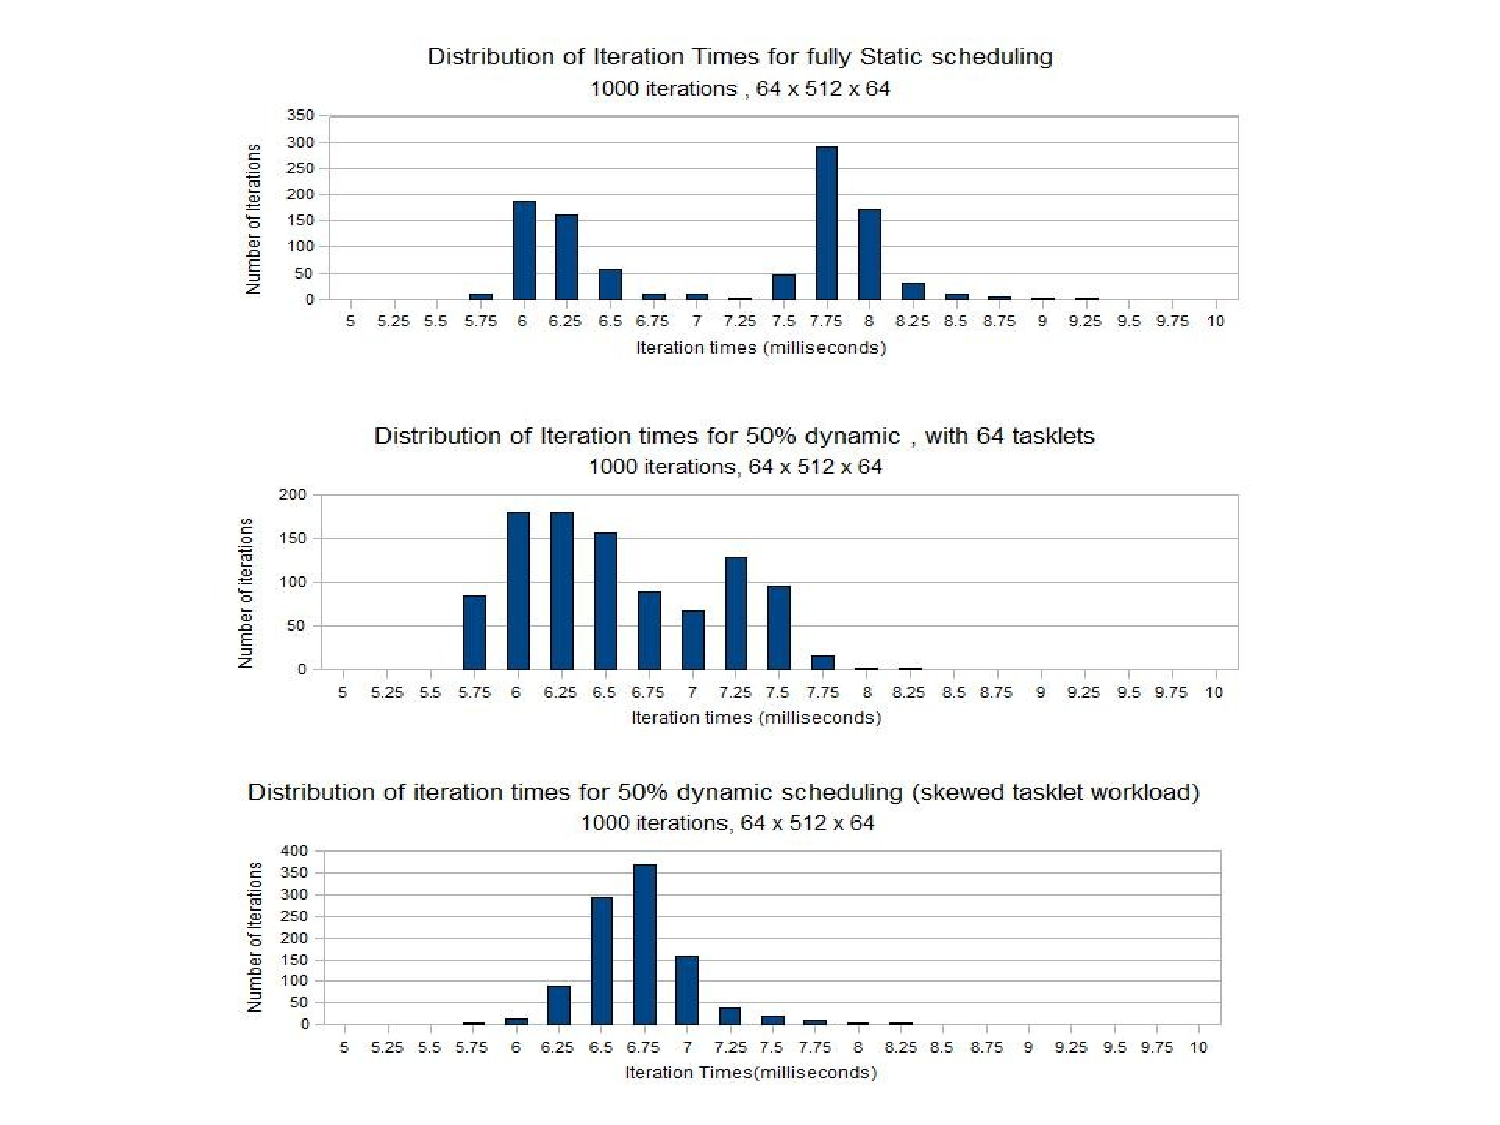
\includegraphics[scale=0.22]{images/uSched-signature-graph}} 
\framebox{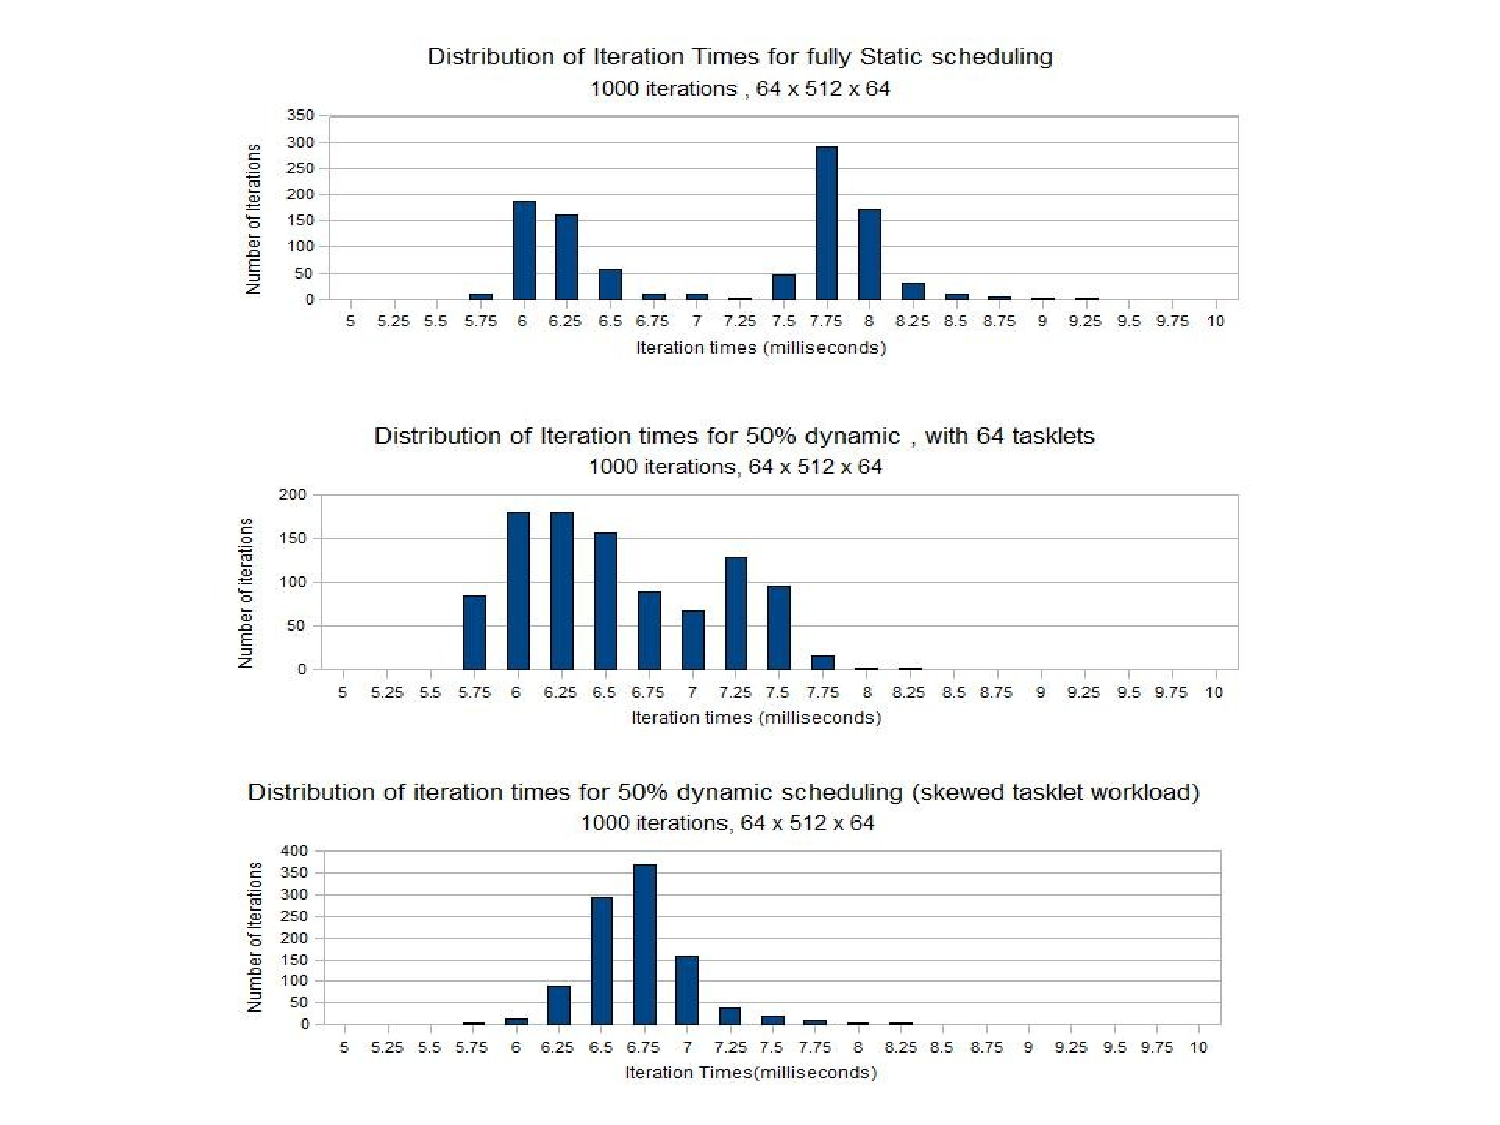
\includegraphics[width=\textwidth]{images/uSched-signature-graph}} 
\end{columns} 
\end{frame} 

\begin{frame}
\frametitle{The Noise Amplification Problem}
\begin{itemize}
\item \small Each node has unpredictable, \textit{excess work}, 
which we call ``noise''.  \\ 
\item \small The resulting load imbalance is  \textit{uncoordinated},
  \textit{localized}, and \textit{transient} (U.L.T.).  \\ 
\item \small This noise is negligible for a program running on a
  single node. \\
\begin{itemize} 
\item \small For example, 0.1\% overhead.  
\end{itemize}  

\item However, with dependences in MPI applications, especially via collective communication, 
if one core of a node experiences U.L.T. event in a timestep, the global timestep is slowed 
down. 
\begin{itemize}
\item \small All other nodes wait for the affected node to finish.  
\end{itemize}

\item \small So, as we increase the number of nodes, it becomes increasingly likely that
\textit{some} core will experience a U.L.T. event, in each timestep. 
\item \small The 0.1\% overhead becomes amplified to a much larger fraction. 
\begin{itemize}
\item \small depending on the amplitude of the U.L.T. event,
and the duration of the application timestep. 
\end{itemize}

%\item \small Given the chain of dependences in MPI collective communication. \\  
%Fundamentally, this U.L.T. load imbalance 
%within each node (or MPI process) during a timestep 
%can \textit{amplify} across nodes, particularly 

%\item \small This amplification can occur within every timestep at very
%  large scale.
% \item \small This is due to the very high likelihood that at least one node
% will suffer a noise event. \\  
% \item \small This is the noise amplification problem.

\end{itemize}
\end{frame} 

%If we assume that one MPI process handles a node, and within that
%process, we subscribe one thread per core, then we can say that the
%load imbalance is localized within an MPI process. 
%\item \small This excess work is
%  different nodes of a cluster.  
%\item \small This uncoordinated excess work that occurs with some
%  probability induces what we refer to \textit{transient} as 
%opposed to \textit{periodic} load imbalance. 
% \item \small This U.L.T. load imbalance 
induces the {noise amplification problem}, in 
% which small localized load imbalances are amplified globally. 

\begin{frame}
\frametitle{Our Core $\mu$-scheduling Solution: Motivation} 
\begin{itemize}
\item Exploit multiple cores on a node: distribute the excess work on 
the core affected by noise to the other cores dynamically. 
\begin{itemize}
\item {\small Create \textit{tasklets} and schedule them dynamically.} 
\end{itemize} 
\item Optimizations: 
\begin{itemize}
\item {\small Making all work dynamic has high overhead
 (enqueue/dequeue, lock). Thus, we make last fraction 
of work dynamic (the rest is static).}
\item {\small Dynamic scheduling interferes with locality across timesteps.
Thus, we keep track of the core that executed it last iteration, and try to keep work on that core. }
\end{itemize} 
\end{itemize}
\end{frame} 

\begin{frame}
\frametitle{MPI Domain Decomposition for 3D Stencil} 
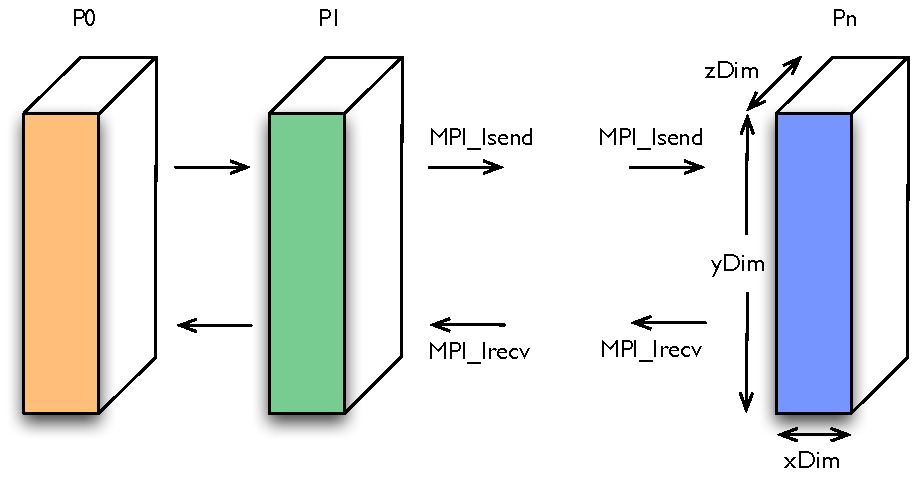
\includegraphics[width=\textwidth]{images/mpi_decomp}
\end{frame} 

\begin{frame} 
\frametitle{Using Our Core $\mu$-scheduling Solution} 
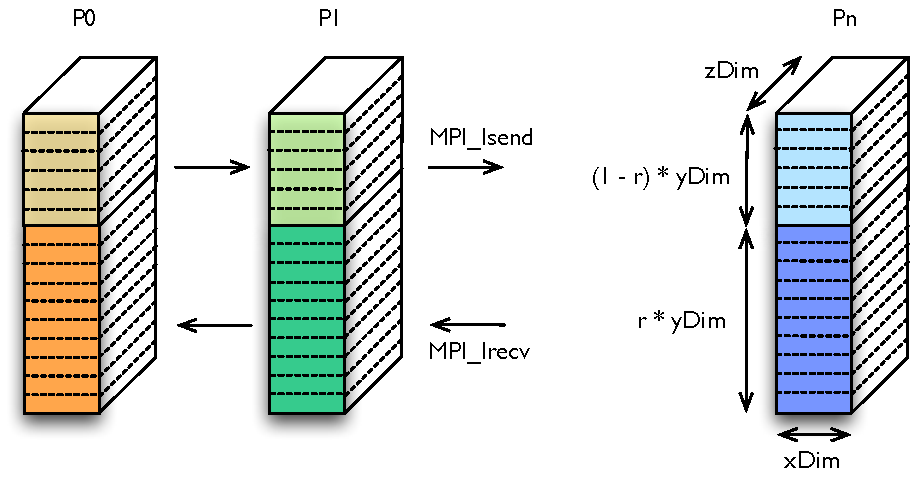
\includegraphics[width=\textwidth]{images/hybrid_decomp}
\end{frame} 

\begin{frame}
\frametitle{What this $\mu$-scheduler Gives Us} 
% alternative top-align that's better for graphics 
% \framebox{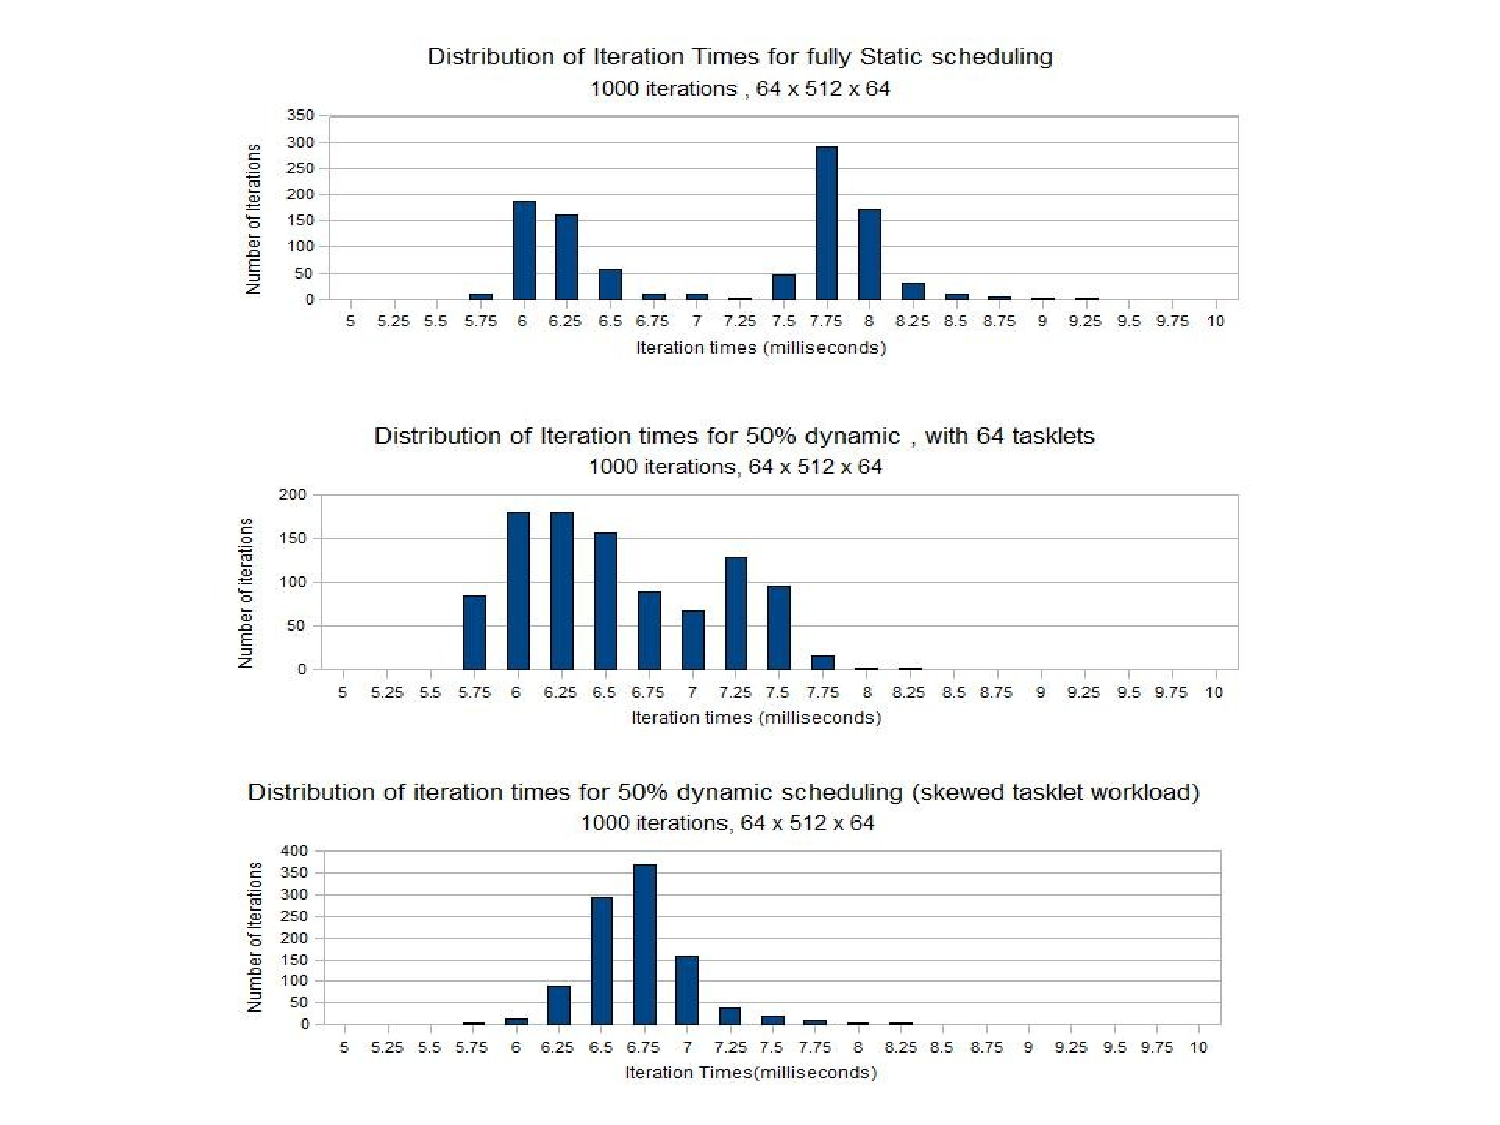
\includegraphics[scale=0.22]{images/uSched-signature-graph}} 
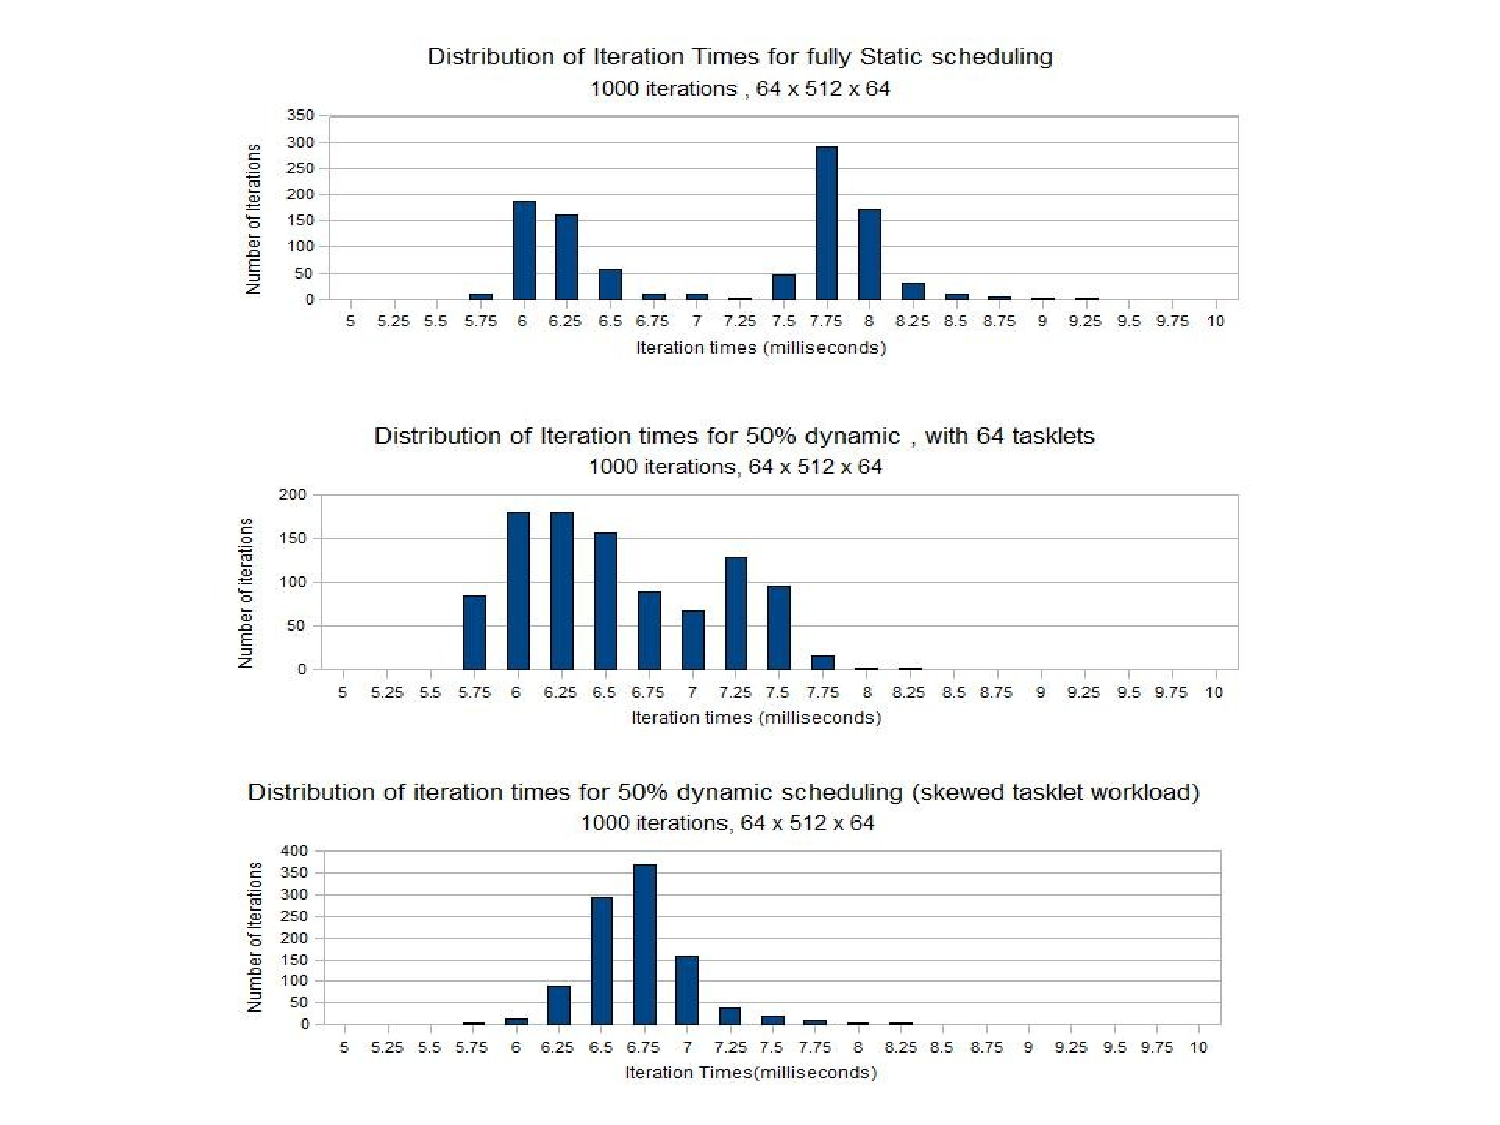
\includegraphics[width=\textwidth]{images/uSched-signature-graph} 
%\end{columns} 
\end{frame} 

%\begin{frame}[Problem and Benefits of Basic Solution]
%\centering \frametitle{Problem and Benefits of Our Basic Solution}  
%\framebox{\includegraphics[width=0.50\textwidth]{ProblemHisto}}
%\centering \framebox{\includegraphics[width=0.30\textwidth]{JitterImpactSkewedWorkLoads}}
%\end{frame} 

%\begin{frame}[A close look at noise spread across cores]
%\frametitle{Noise characterization of Jaguar}
%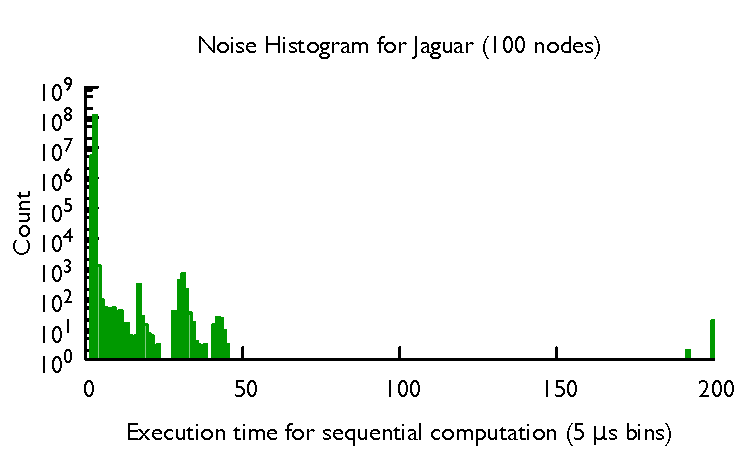
\includegraphics[width=\textwidth]{images/noise_shist_jaguar}
%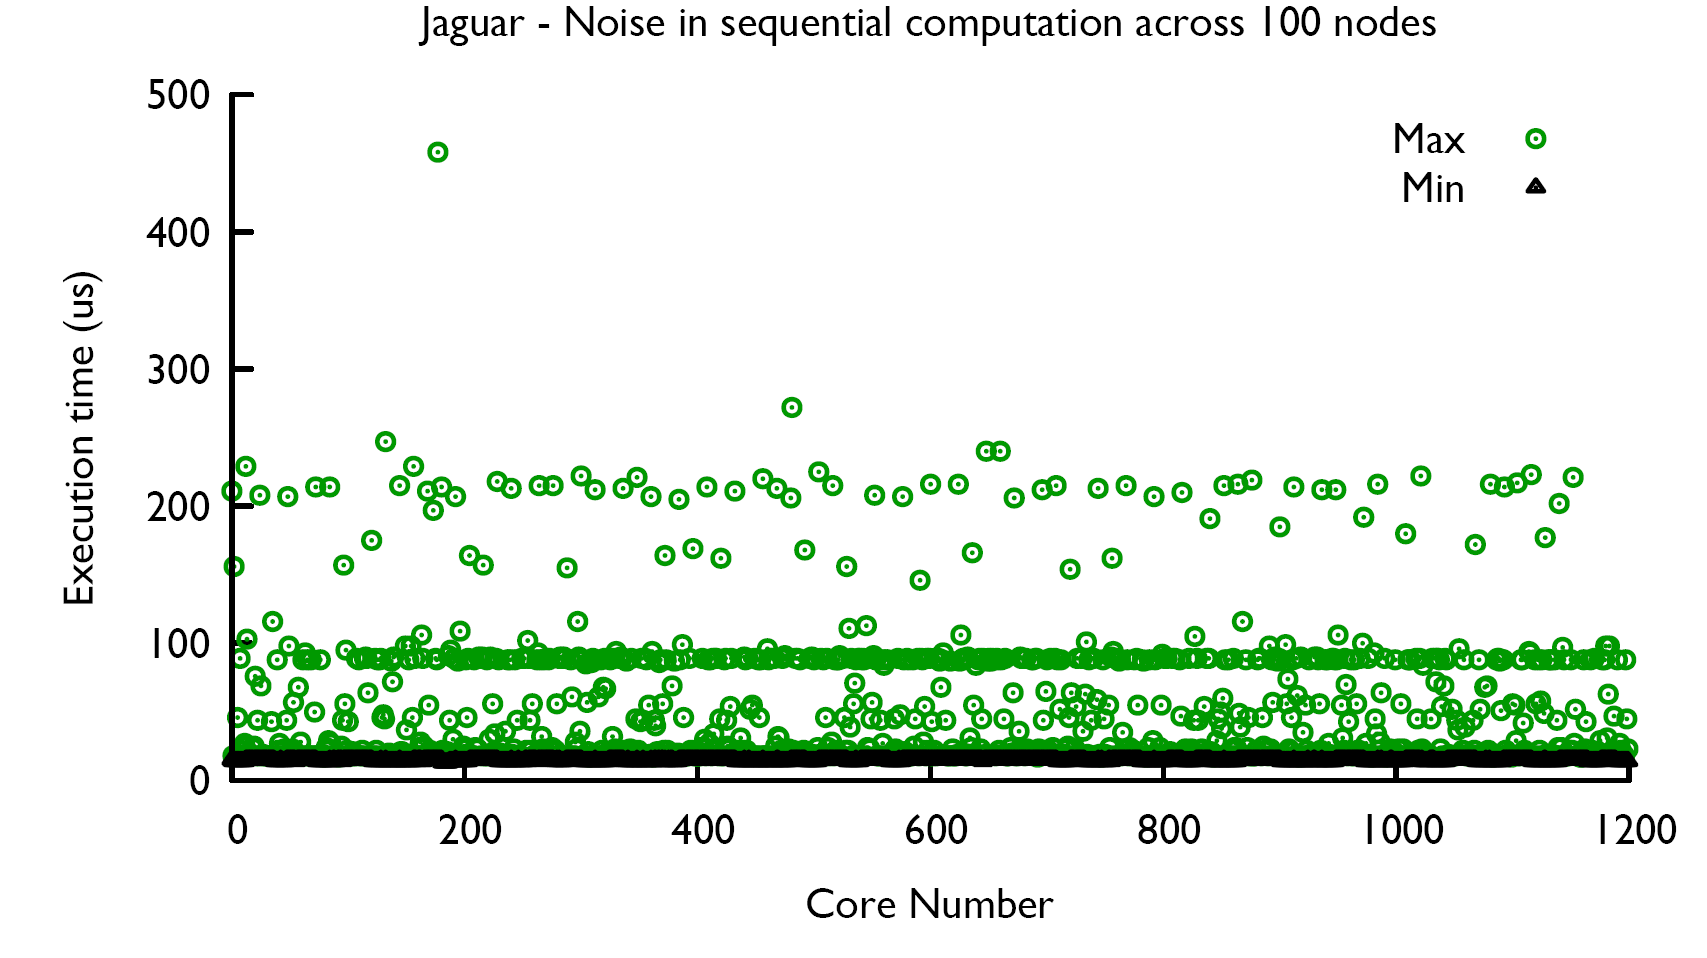
\includegraphics[width=\textwidth]{images/NoiseJaguar}
%\end{frame}

%\begin{frame}[A close look at noise spread across cores]
%\frametitle{Noise characterization of Ranger}
%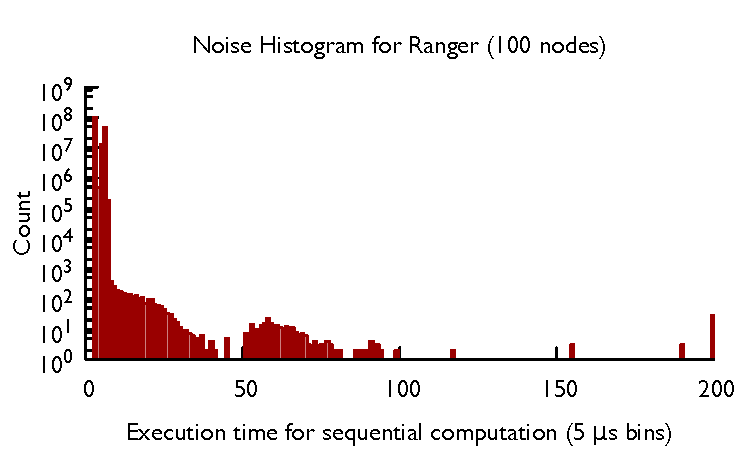
\includegraphics[width=\textwidth]{images/noise_shist_ranger}
%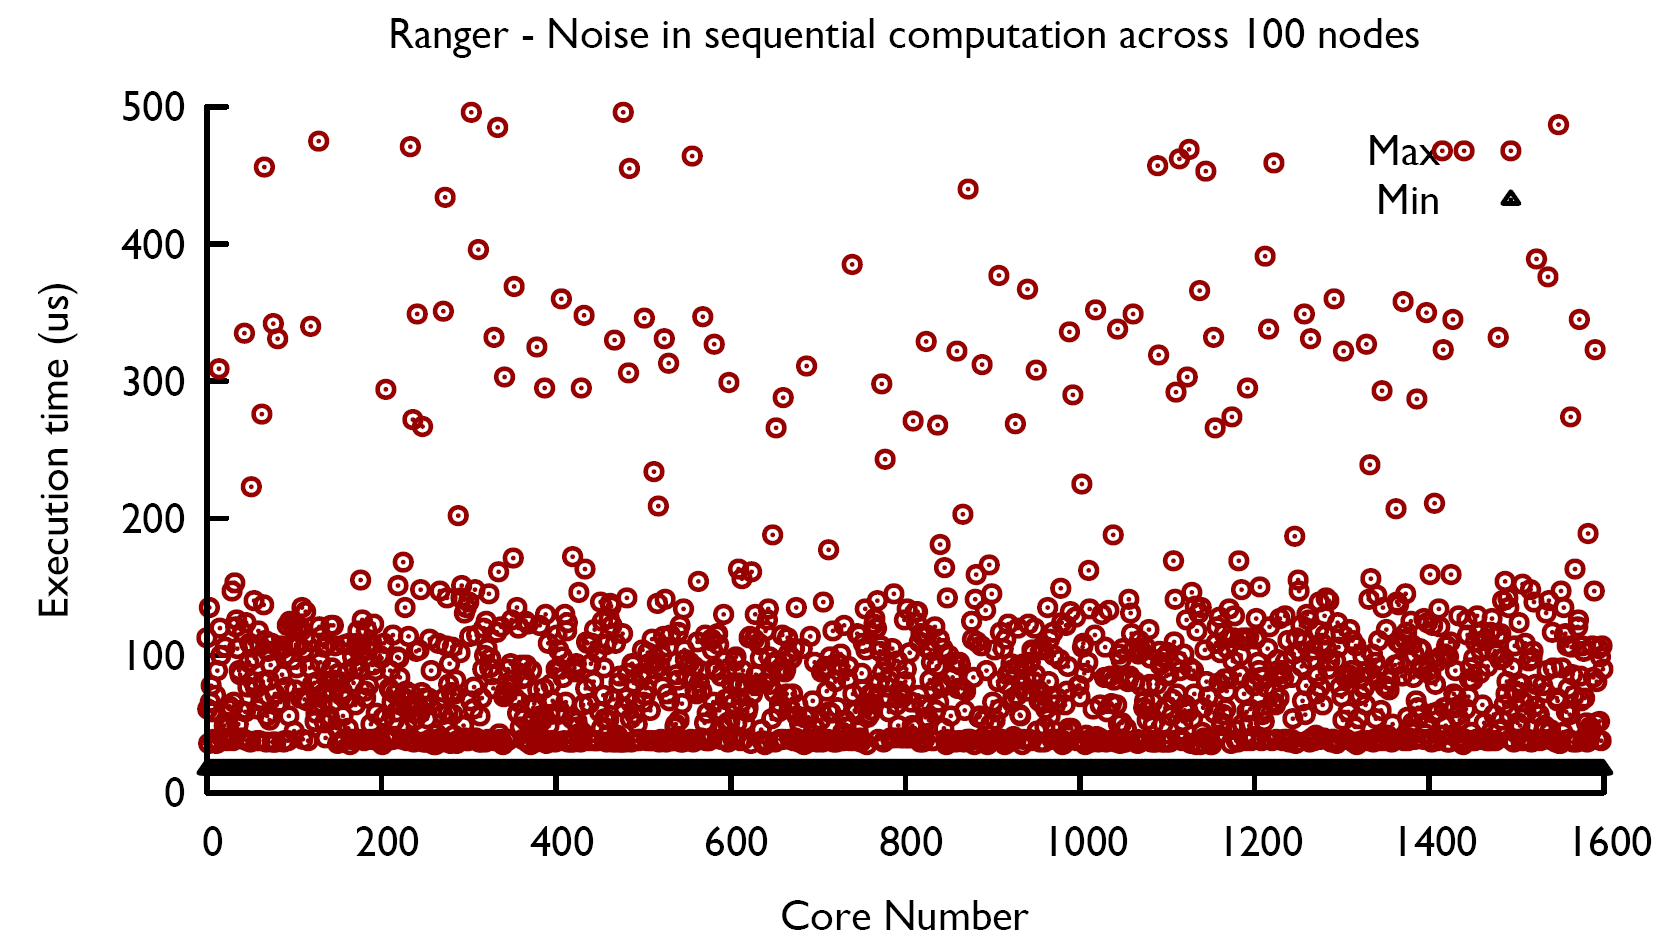
\includegraphics[width=\textwidth]{images/NoiseRanger}
%\end{frame}

\begin{frame}[A Close Look at Noise spread across cores]
\frametitle{Noise Characteristics on Two Supercomputers}
\begin{columns}
\column{0.5\textwidth}
\centering \textbf{Jaguar} \\
%\framebox{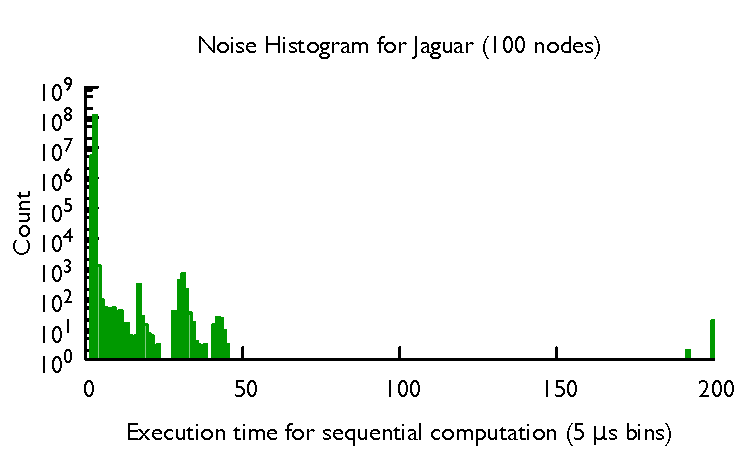
\includegraphics[width=\textwidth]{images/noise_shist_jaguar}}
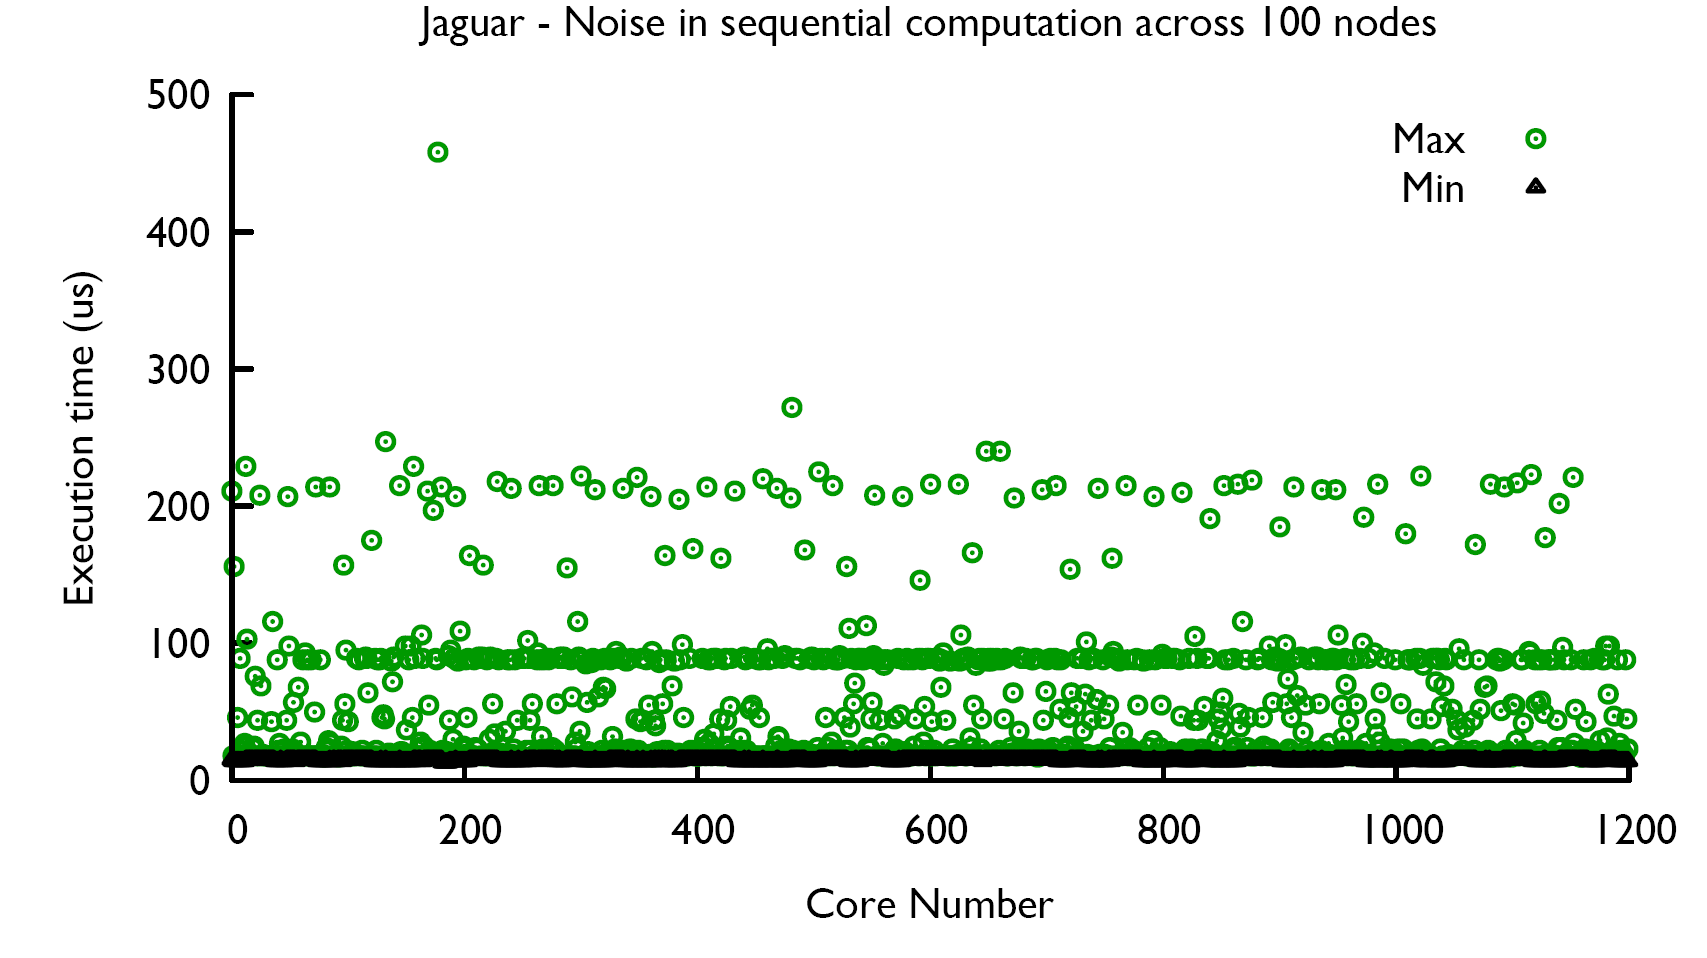
\includegraphics[width=\textwidth]{images/NoiseJaguar} 
%\includegraphics[width=\textwidth]{images/NoiseSignatures-Jaguar}
\column{0.5\textwidth}
\centering \textbf{Ranger} \\
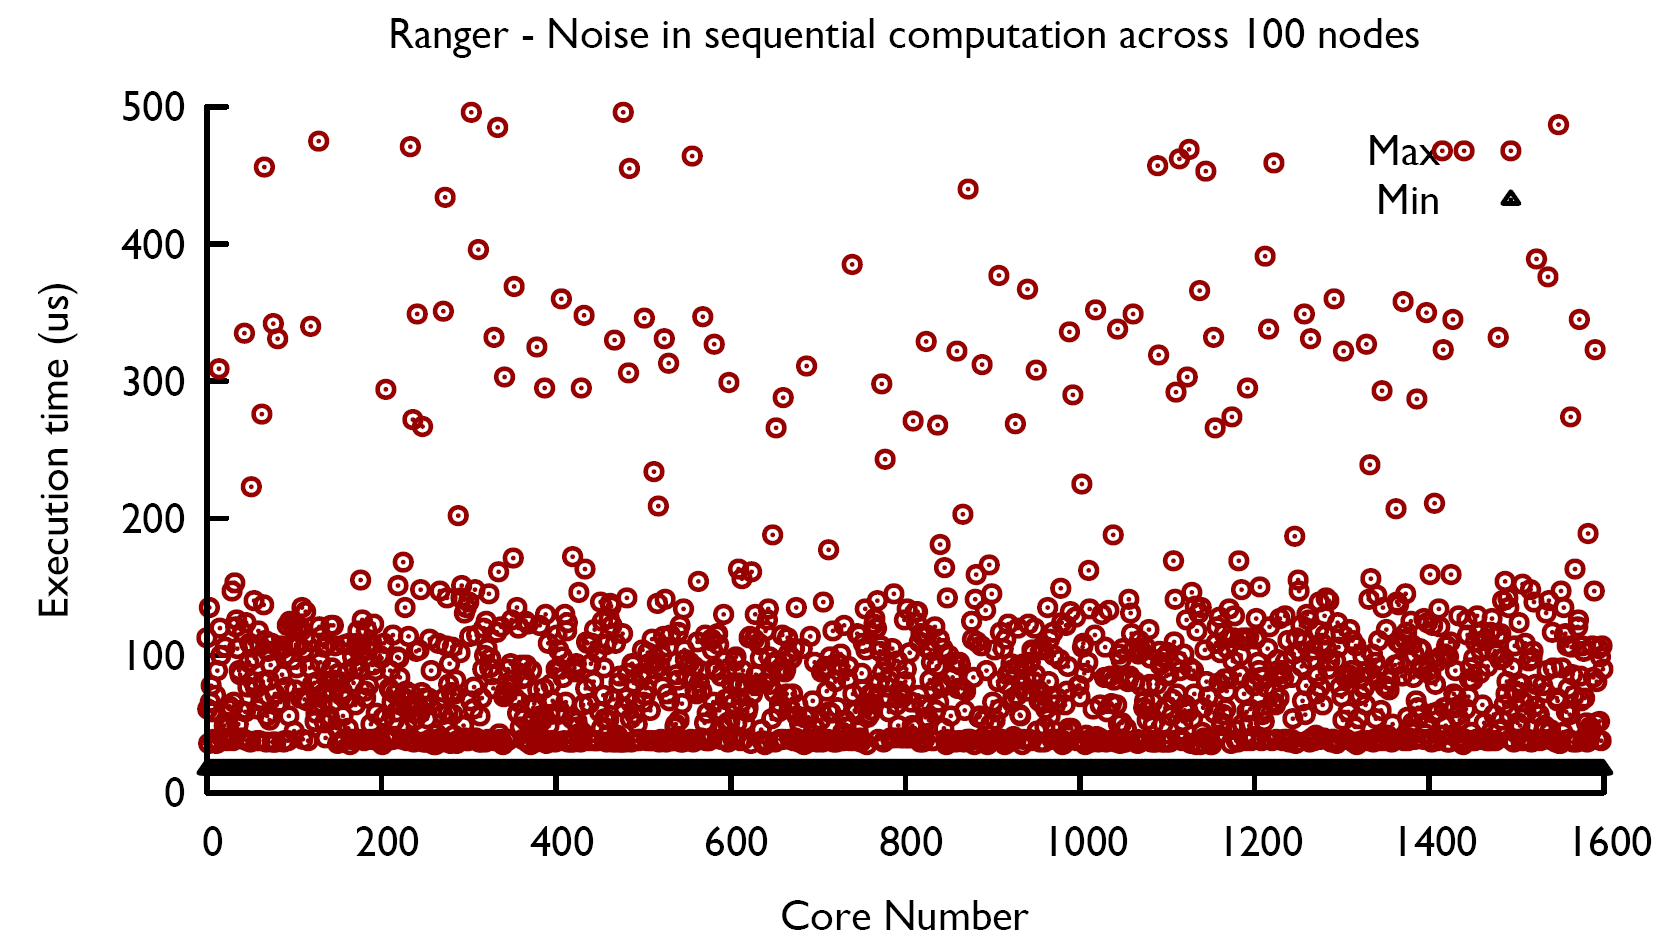
\includegraphics[width=\textwidth]{images/NoiseRanger} 
%\includegraphics[width=\textwidth]{images/NoiseSignatures-Ranger} 
%\framebox{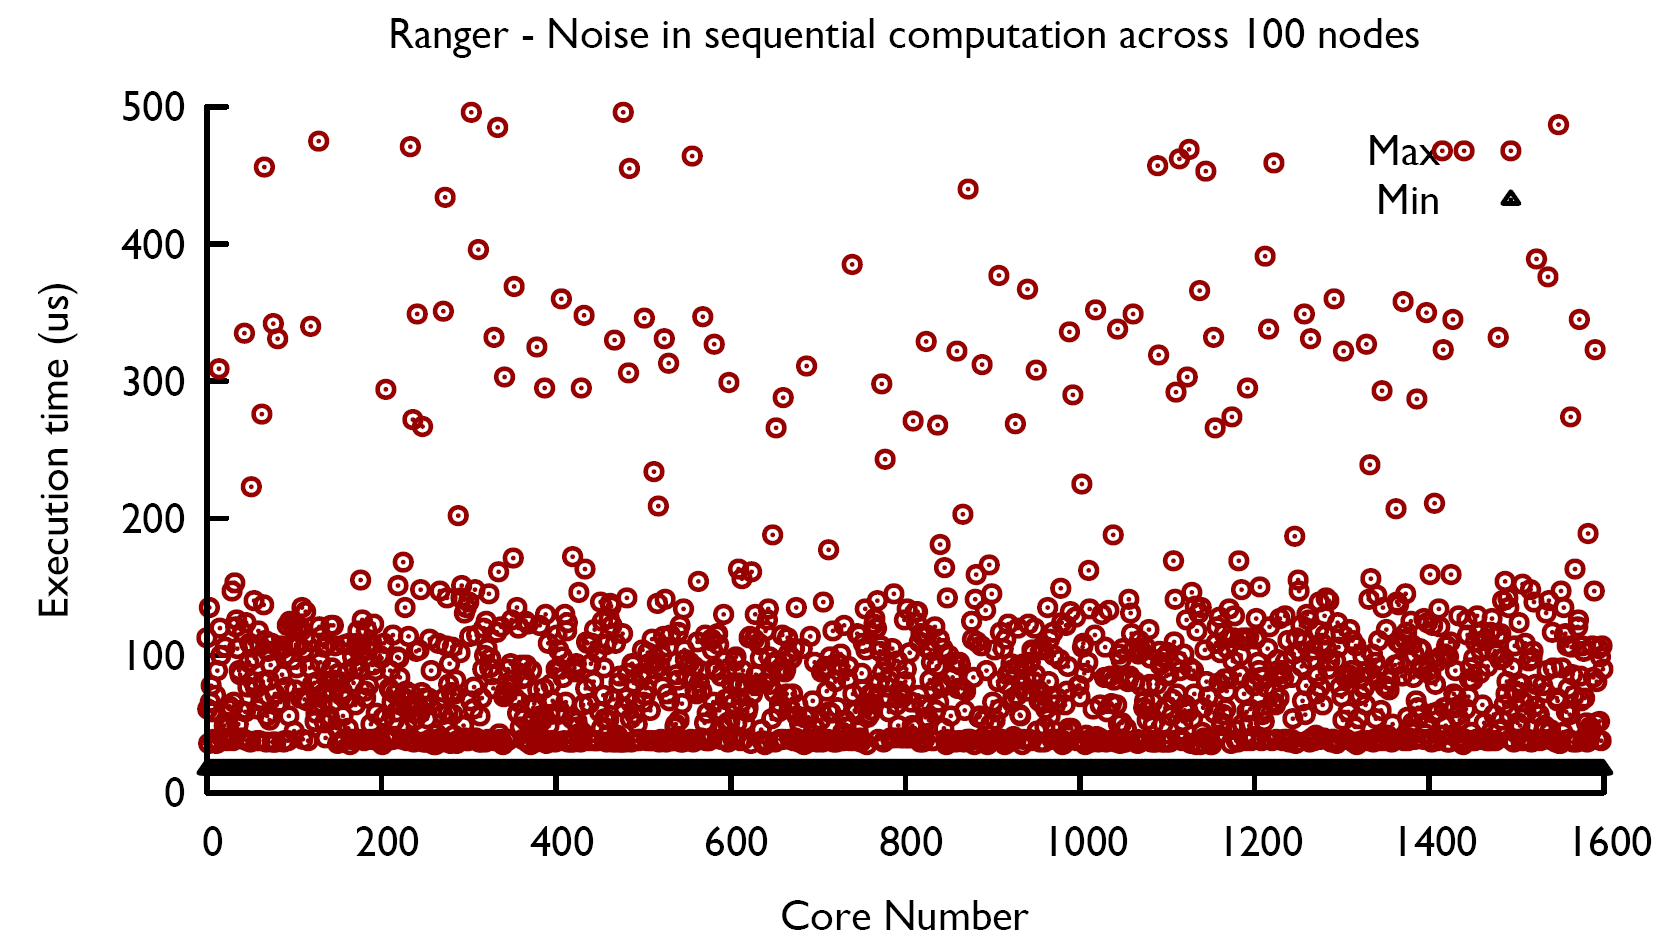
\includegraphics[width=\textwidth]{images/NoiseRanger}} 
\end{columns} 

Some of the noise is high frequency (occurs in every timestep on every
node), and confined to a subset of cores on each node. 

\textbf{Could we use this knowledge to improve scheduler? } 
\end{frame} 

\begin{frame}[A Close Look at Noise spread across cores]
\frametitle{Noise Characteristics on Two Supercomputers}
\begin{columns}
\column{0.5\textwidth}
\centering \textbf{Jaguar} \\
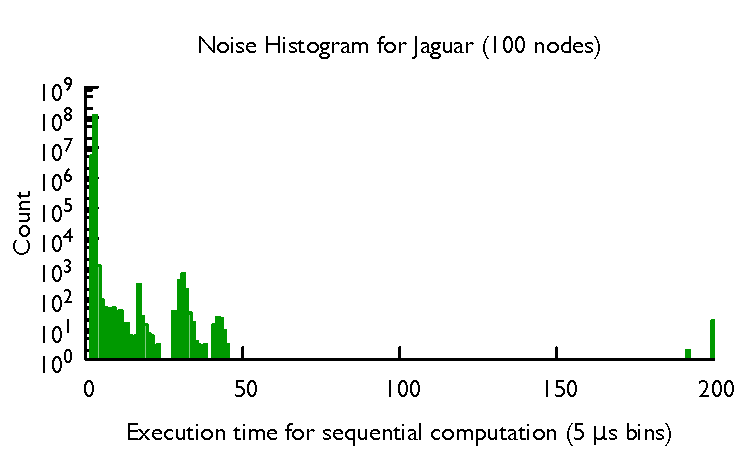
\includegraphics[width=\textwidth]{images/noise_shist_jaguar}
%\framebox{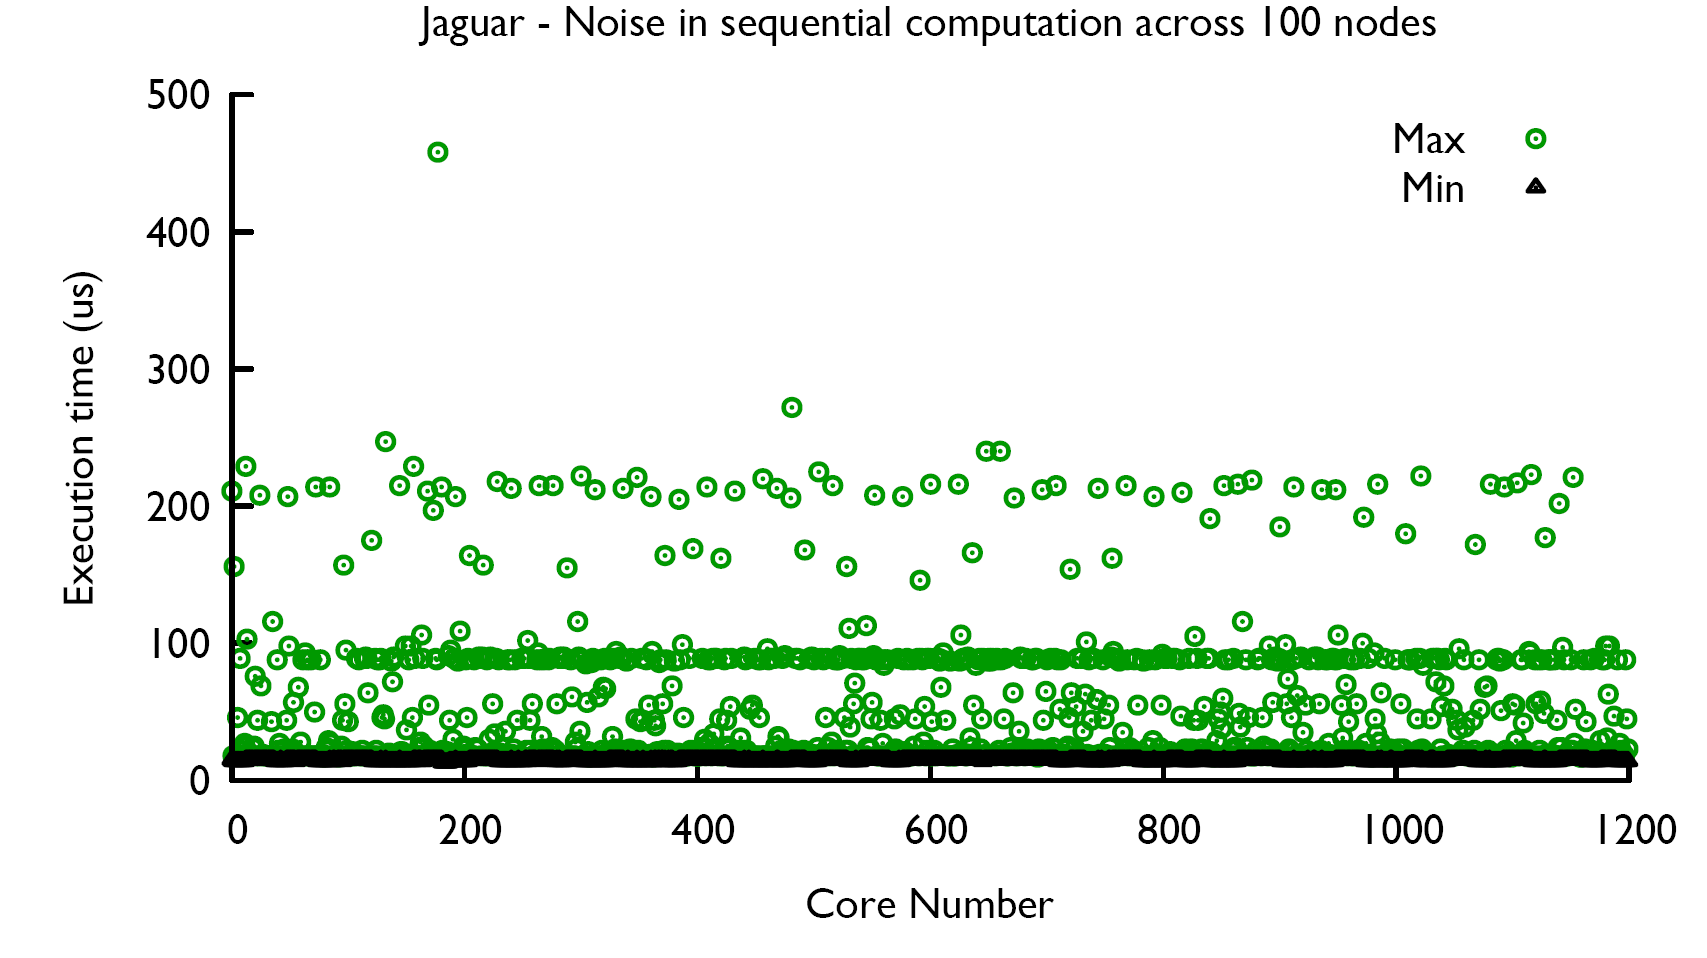
\includegraphics[width=\textwidth]{images/NoiseJaguar}} 
%\framebox{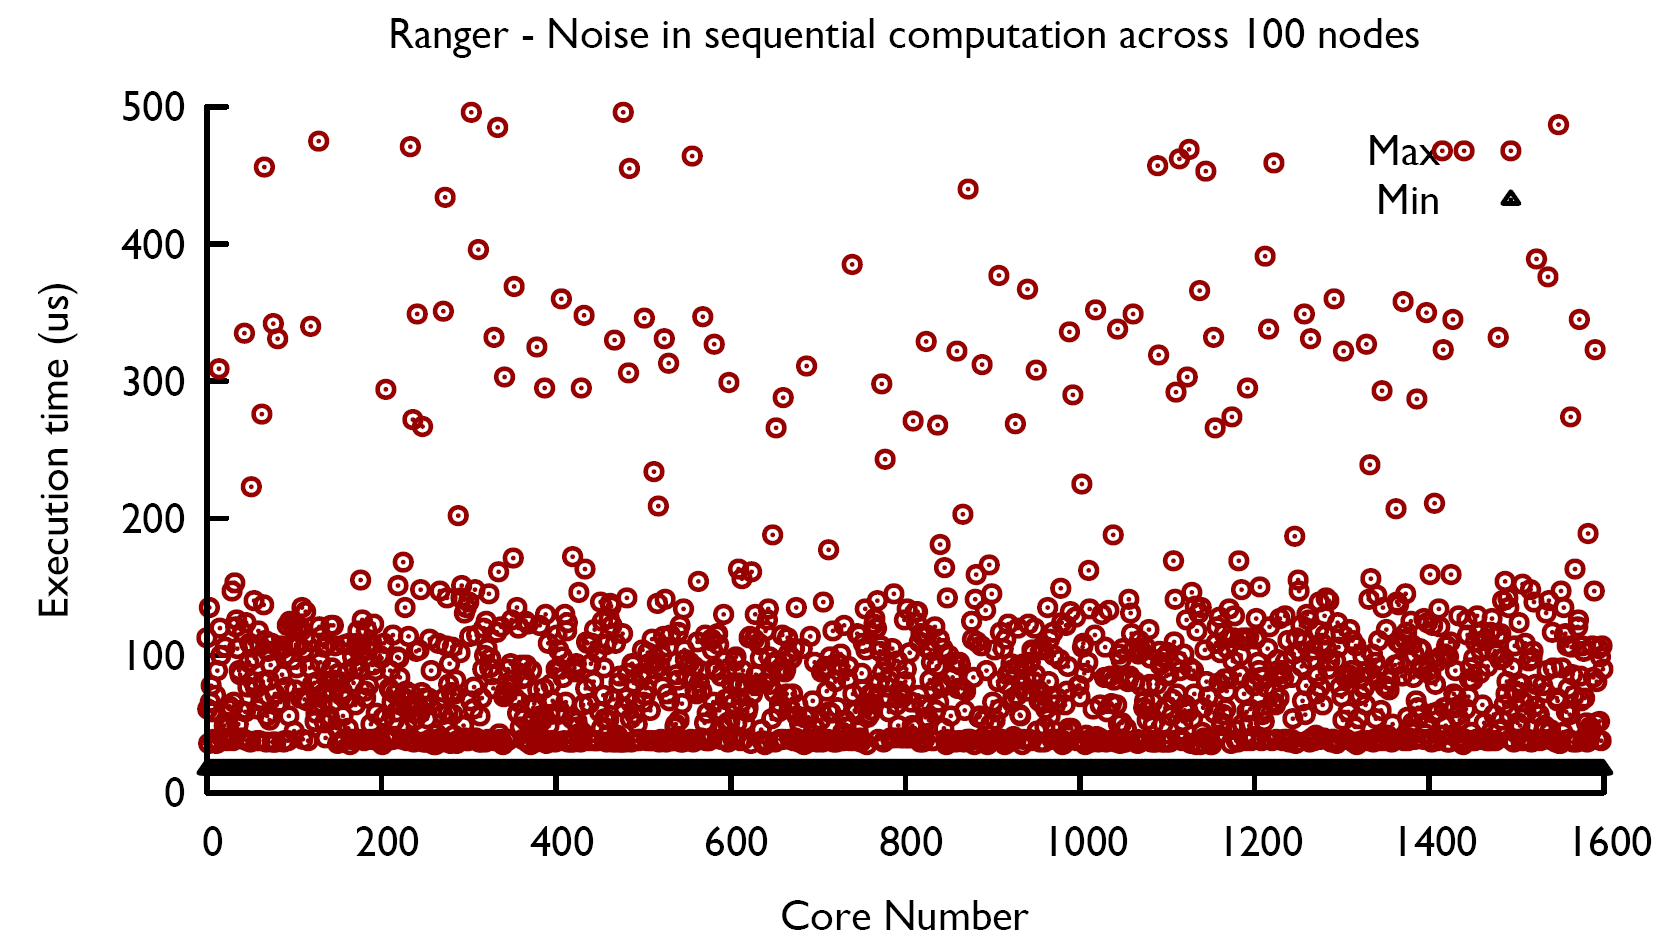
\includegraphics[width=\textwidth]{images/NoiseRanger}} 
\column{0.5\textwidth}
\centering \textbf{Ranger} \\
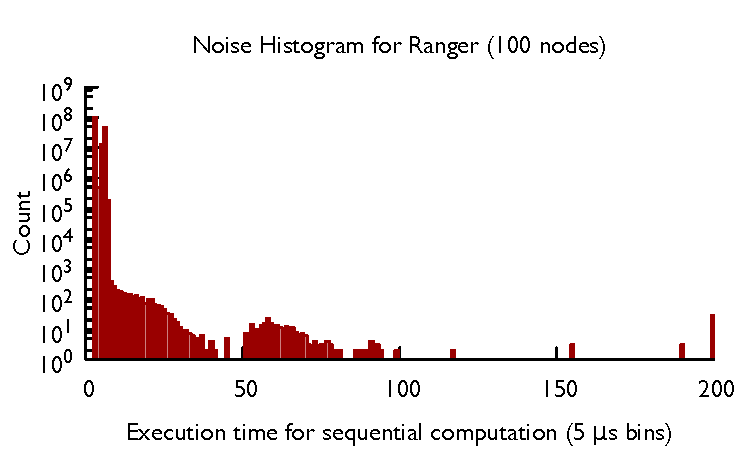
\includegraphics[width=\textwidth]{images/noise_shist_ranger}
%\framebox{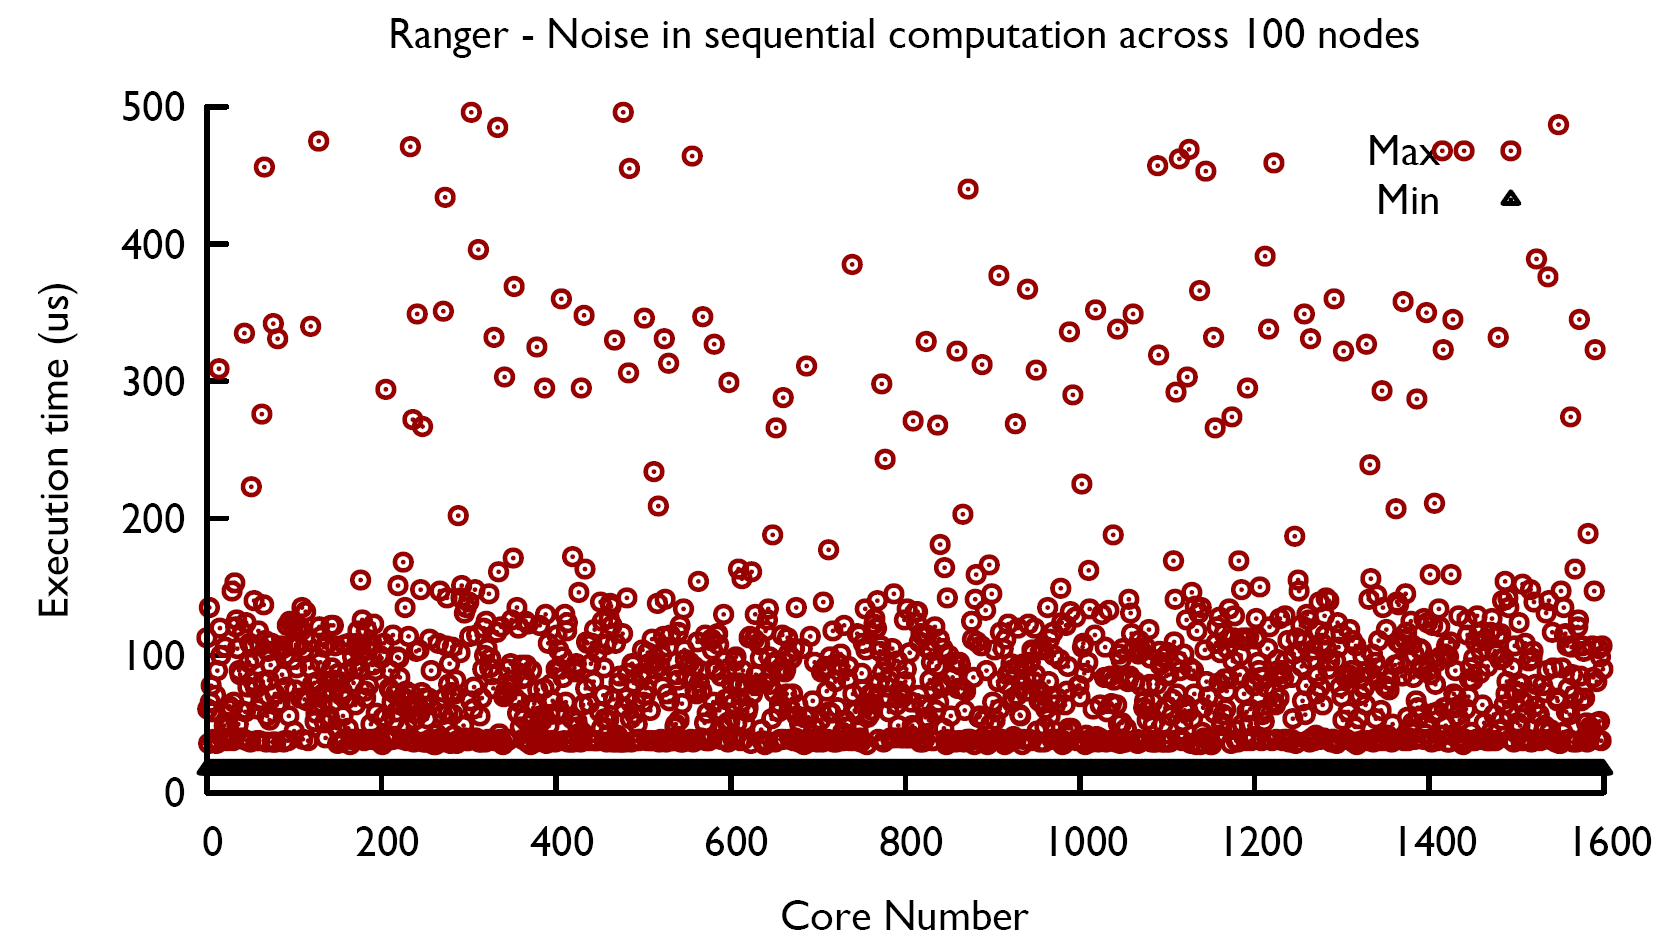
\includegraphics[width=\textwidth]{images/NoiseRanger}} 
%\framebox{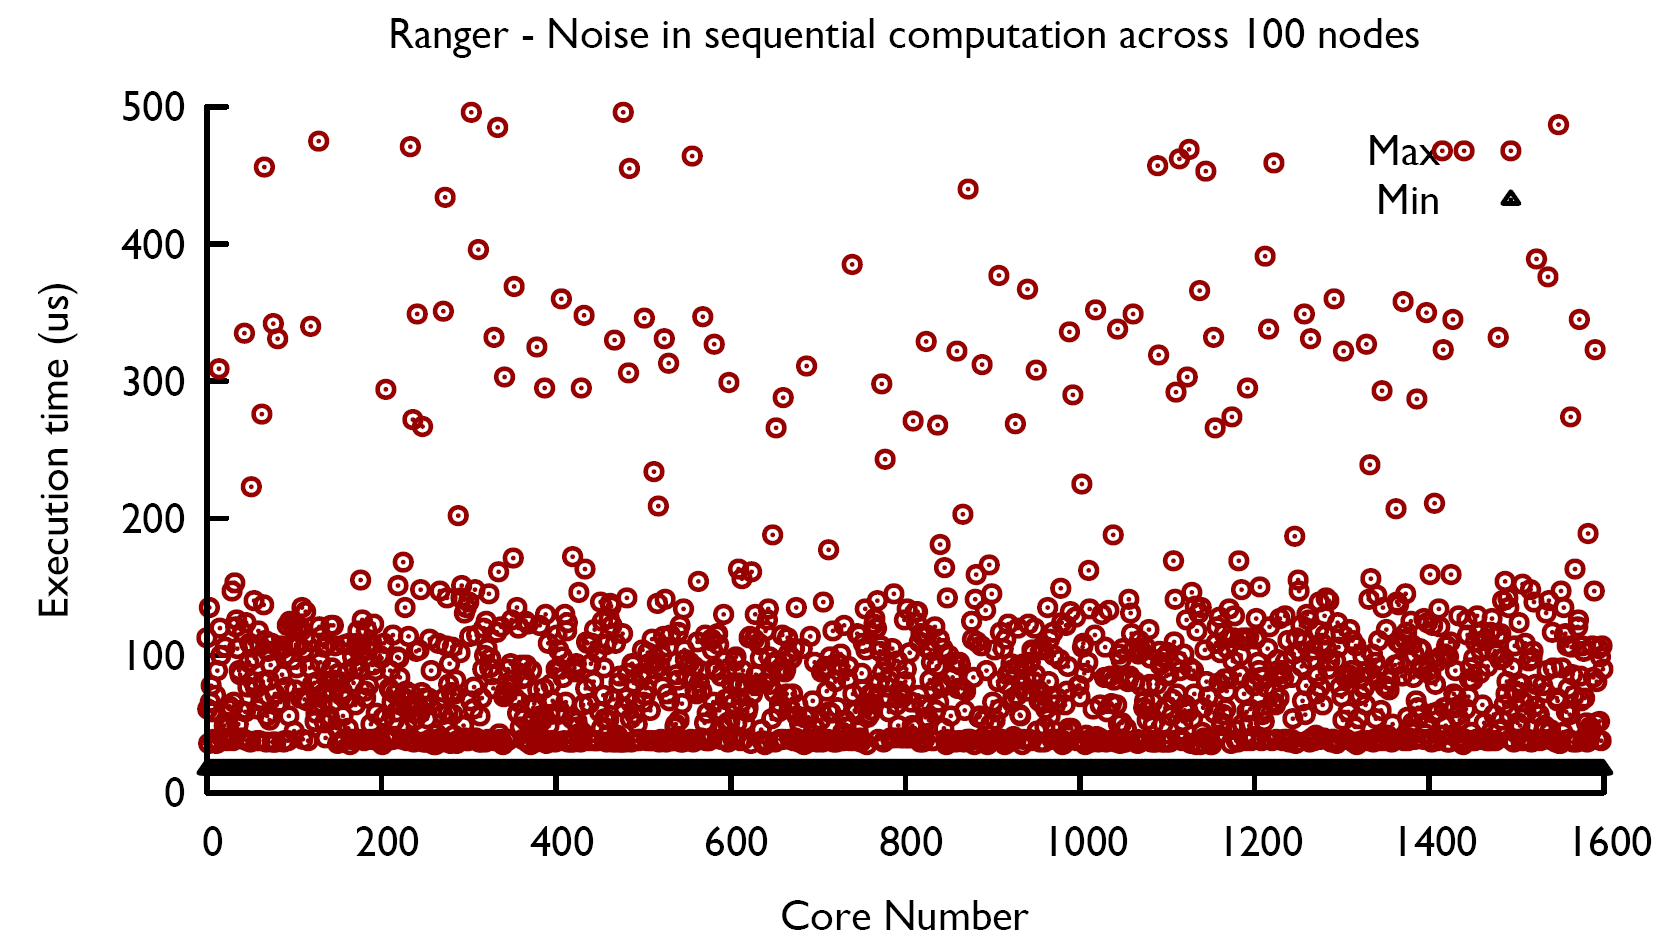
\includegraphics[width=\textwidth]{images/NoiseRanger}} 
\end{columns}
\end{frame} 

%\begin{frame}[A Close Look at Noise Spread Across Cores]
%\frametitle{Noise Characteristics on Two Supercomputers}
%\begin{columns}
%\column{0.5\textwidth}
%\centering \textbf{Jaguar} \\
%\framebox{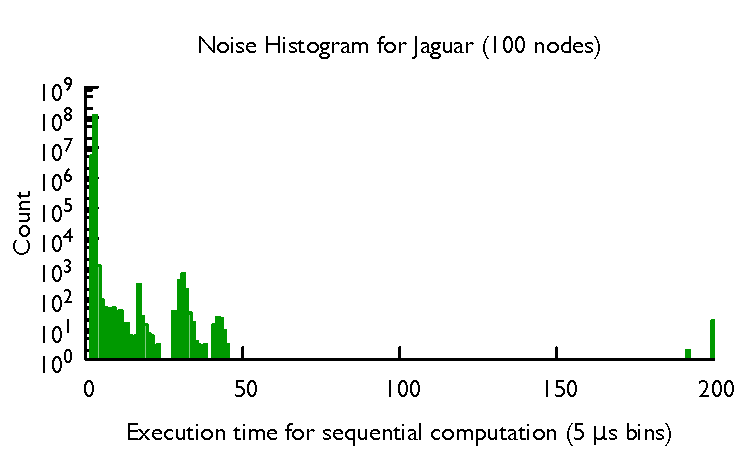
\includegraphics[width=\textwidth]{images/noise_shist_jaguar}}
%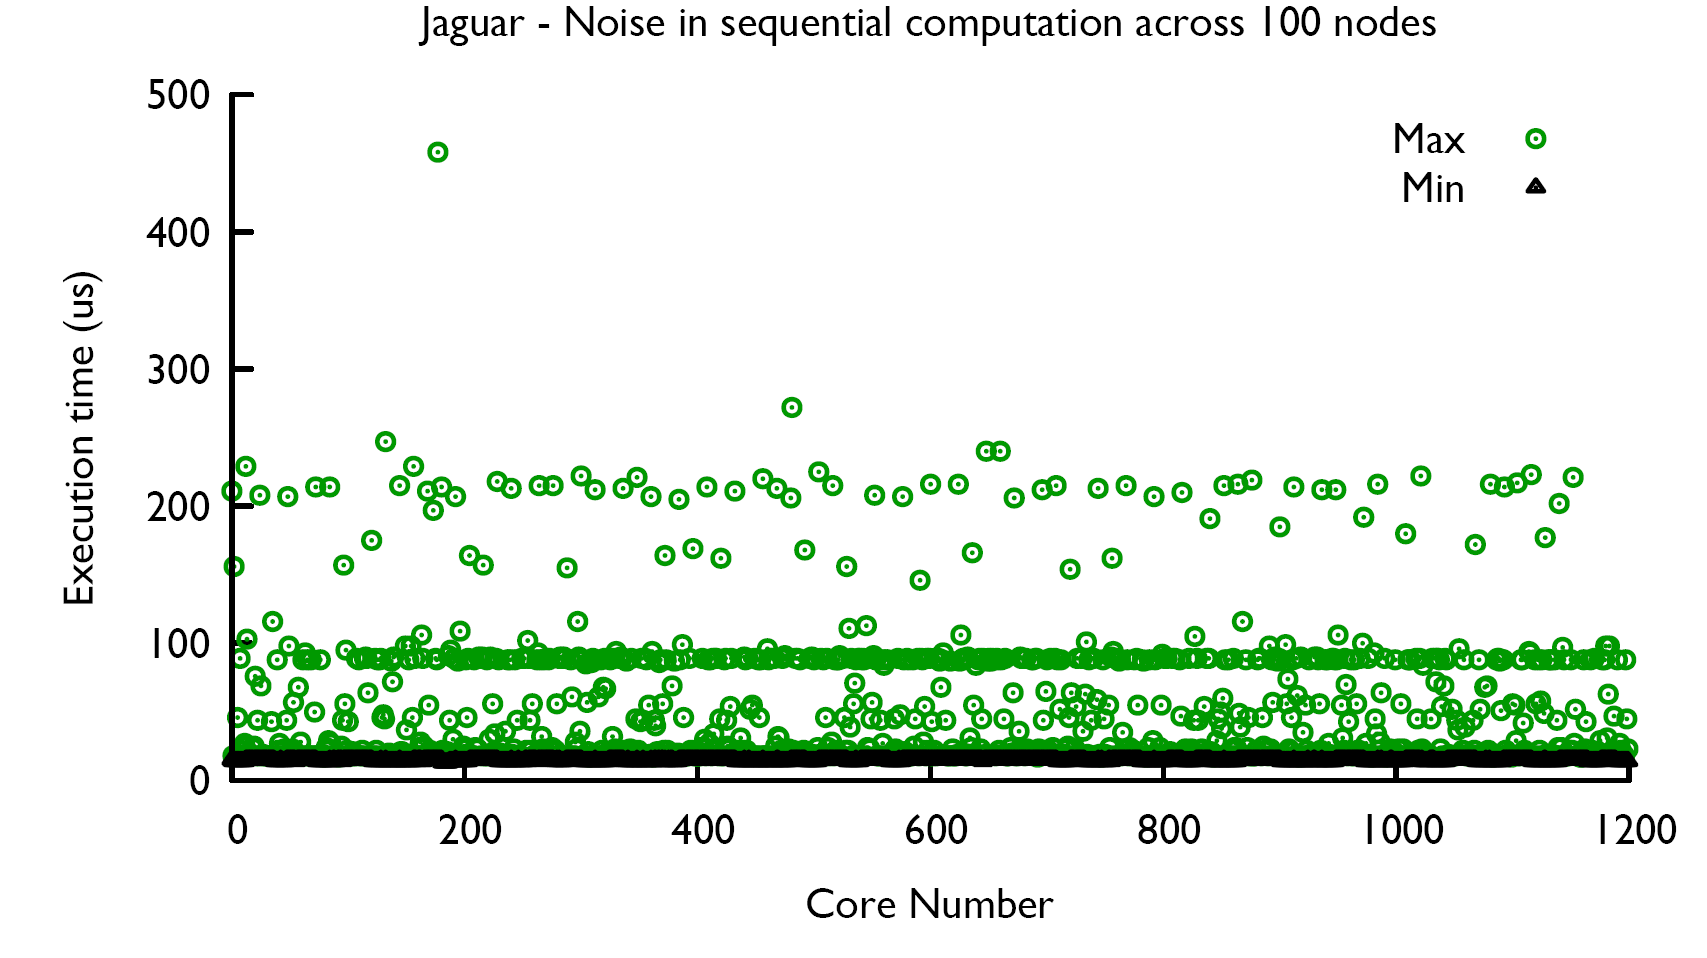
\includegraphics[width=\textwidth]{images/NoiseJaguar} 
%\includegraphics[width=\textwidth]{images/NoiseSignatures-Jaguar}
%\column{0.5\textwidth}
%\centering \textbf{Ranger} \\
%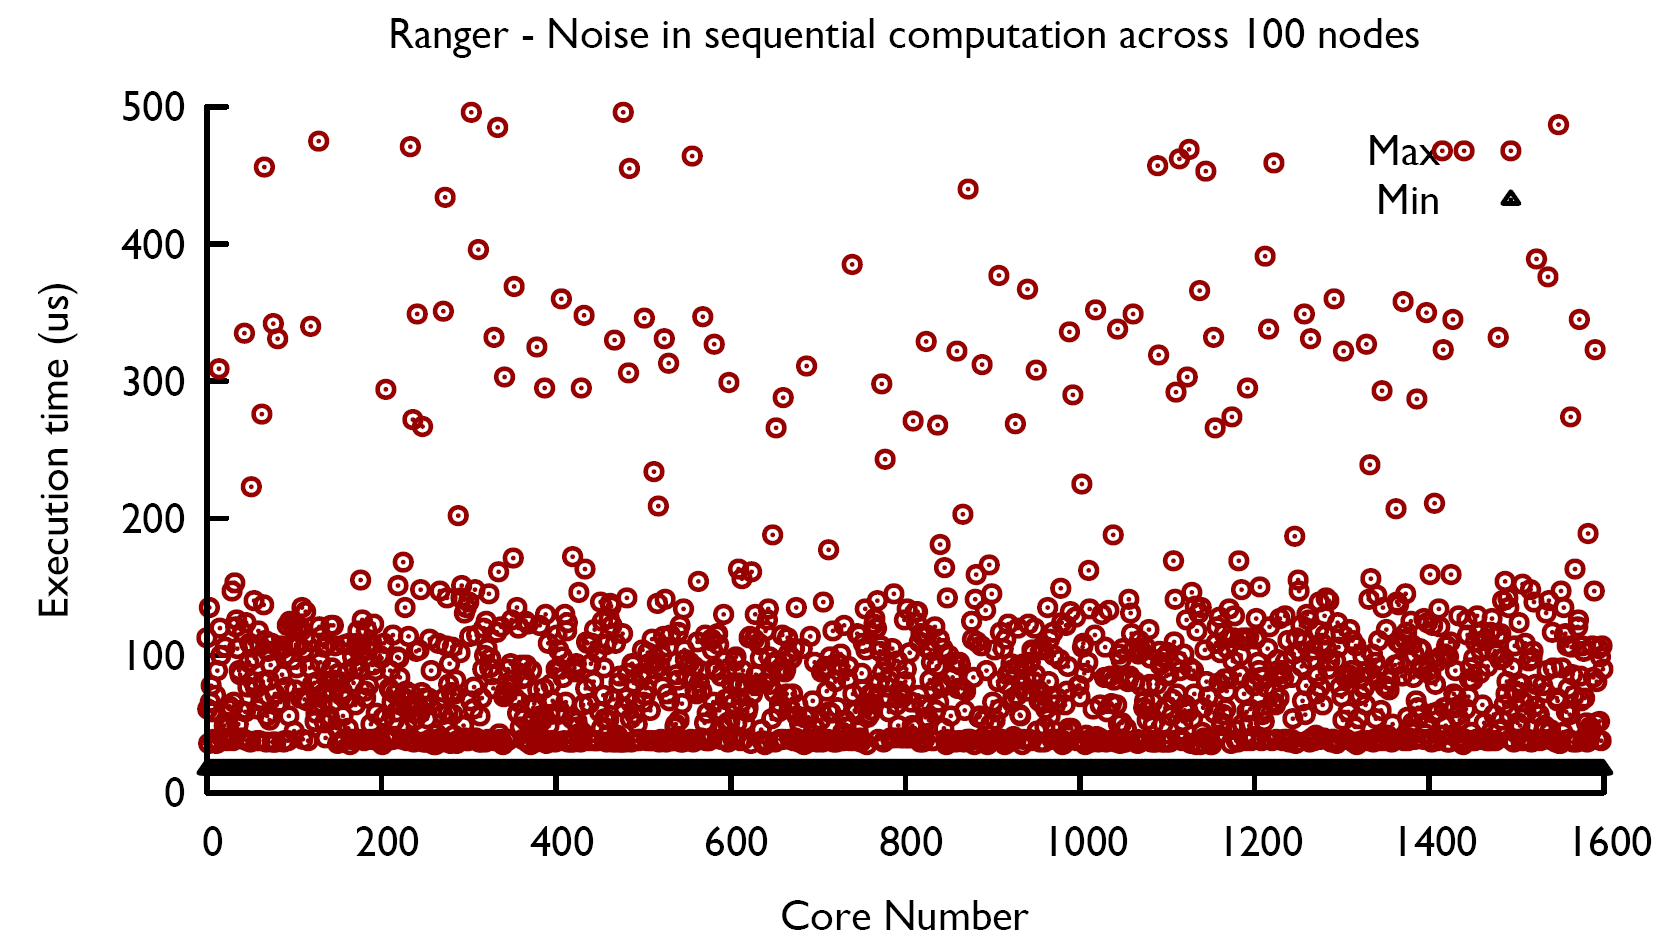
\includegraphics[width=\textwidth]{images/NoiseRanger} 
%\includegraphics[width=\textwidth]{images/NoiseSignatures-Ranger} 
%\framebox{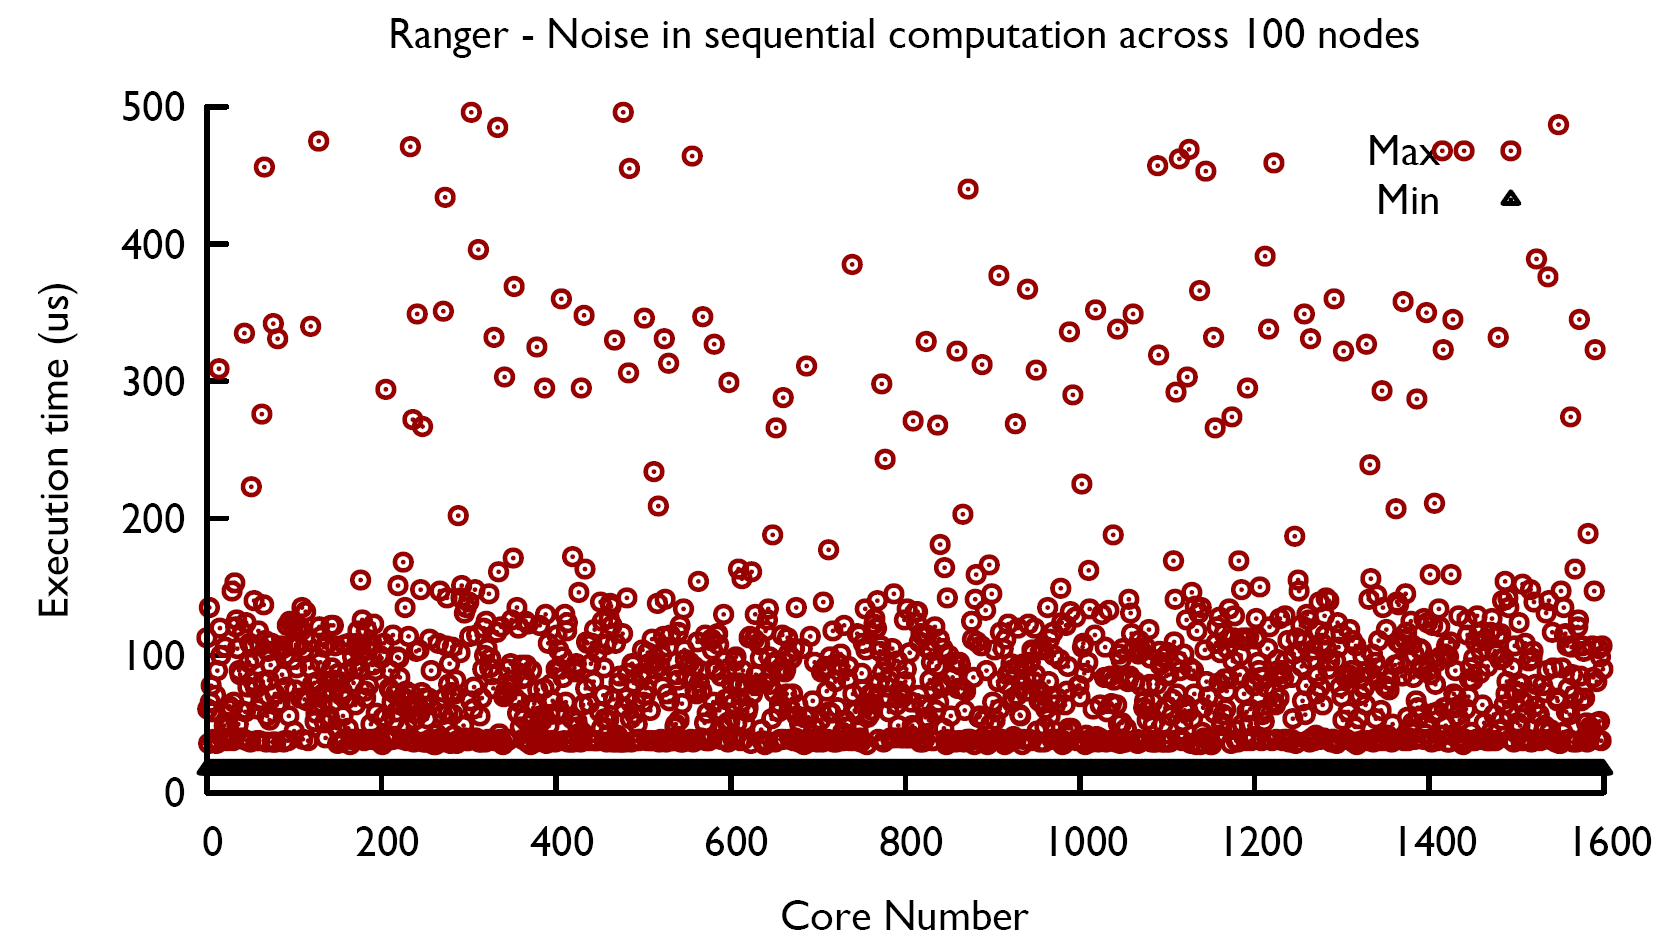
\includegraphics[width=\textwidth]{images/NoiseRanger}} 
%\end{columns} 
%\end{frame}
 
\begin{frame}[Two fundamentally different approaches to Load Balancing] 
\frametitle{Two Very Different Approaches to Load Balancing} 
\begin{itemize} 
\item \small Measurement-based load balancing and work-stealing 
are driven by two different fundamental beliefs about applications and
architecture. \\  
\begin{itemize}
\item \small Work-stealing: ``invisible hand''(reactive). \\ 
\item \small Predictions from past patterns (proactive). \\
\end{itemize} 

\small \item {\small Earlier, we did not take advantage of the
  persistent patterns in noise signatures.} \\ 
\item {\small Given this, the question we ask is:
``Can we develop a measurement-based load balancing scheme that can
help our original scheduler for the issue of persistent U.L.T. load
imbalance?''} \\ 
\end{itemize} 
\end{frame}  

\begin{frame}[Our Weighted u-scheduling Solution]
\frametitle{Our Adaptive lightweight scheduling Solution}
\begin{itemize} 
\item \small Weight the static section based on measurement of FLOP
rate of each core (obtained from previous timestep); do dynamic 
scheduled phase as usual.  

\begin{itemize} 
    \item {\small The faster cores get to do more of their work
      statically (thus, with less overhead).}  
\end{itemize}  

%\item \small Different from original solution because we
%we still tune for the same percentage dynamic in total, 
% allow for adaptive adjustment of the number of tasklets 
%within the timestep when each core can start 
%pulling tasklets from the queue.  

%\item \small Slow cores are allowed to start pulling from queue 
%after finishing just a few statically assigned tasklets.  

%\item \small The fast (unaffected) cores pull additional statically
% assigned tasklets. 

\item \small Weighted factoring, in conjunction to 
original $\mu$-scheduling, can be of benefit when 
there are a mixture of the two different types of 
load imbalances. 

% high-frequency, 
%low amplitude excess work that spans multiple timesteps
%and low-probability, high amplitude excess work that is within one
%timestep.
\end{itemize} 
\end{frame} 

\begin{frame}
\frametitle{Adaptive $\mu$-Scheduling}
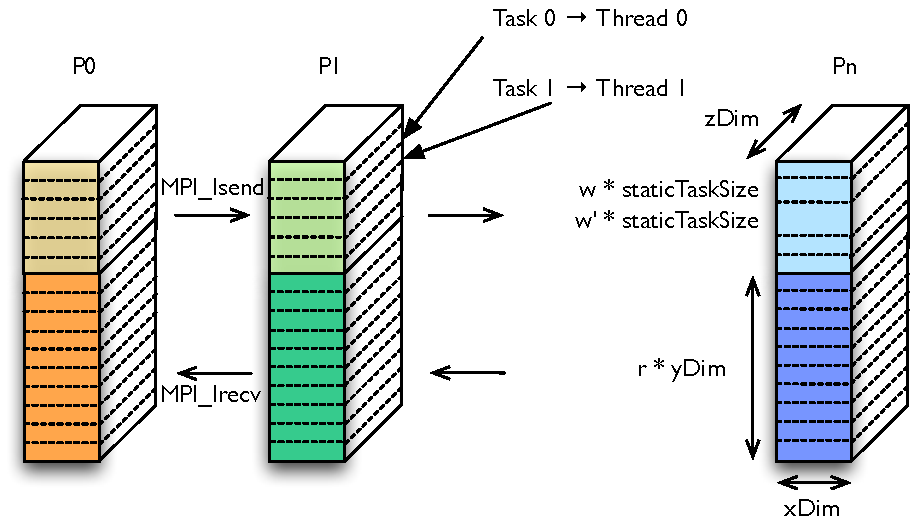
\includegraphics[width=\textwidth]{images/weighted_decomp} 
\end{frame}  

\begin{frame}  
\frametitle{Solution Summary} 
\begin{columns}
\column{0.33\textwidth} 
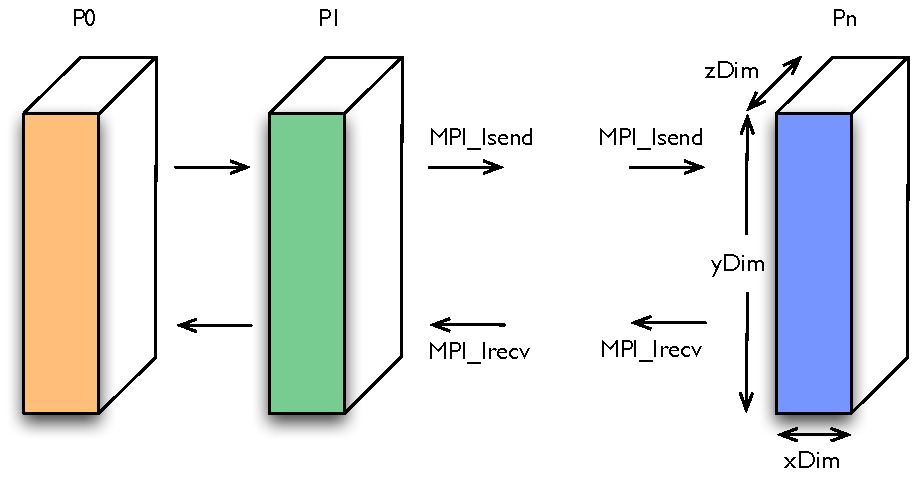
\includegraphics[width=\textwidth]{images/mpi_decomp}
Original 
\column{0.33\textwidth}
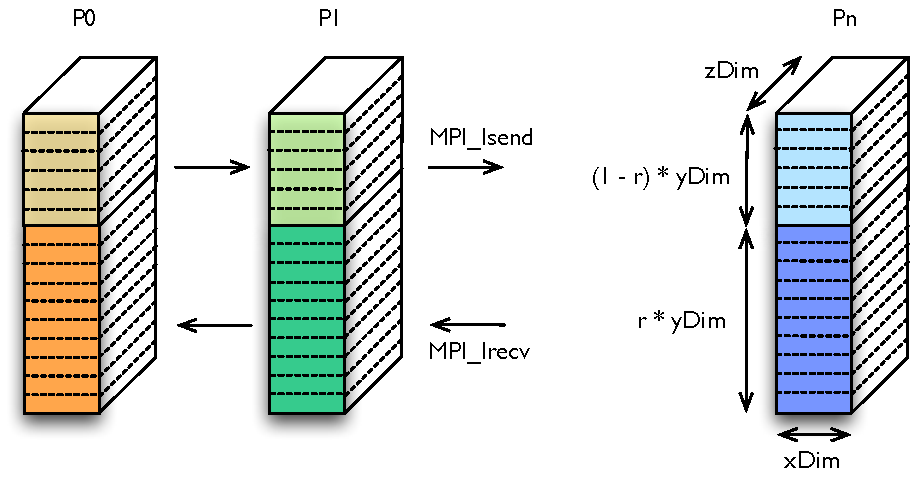
\includegraphics[width=\textwidth]{images/hybrid_decomp}
$\mu$-sched 
\column{0.33\textwidth}
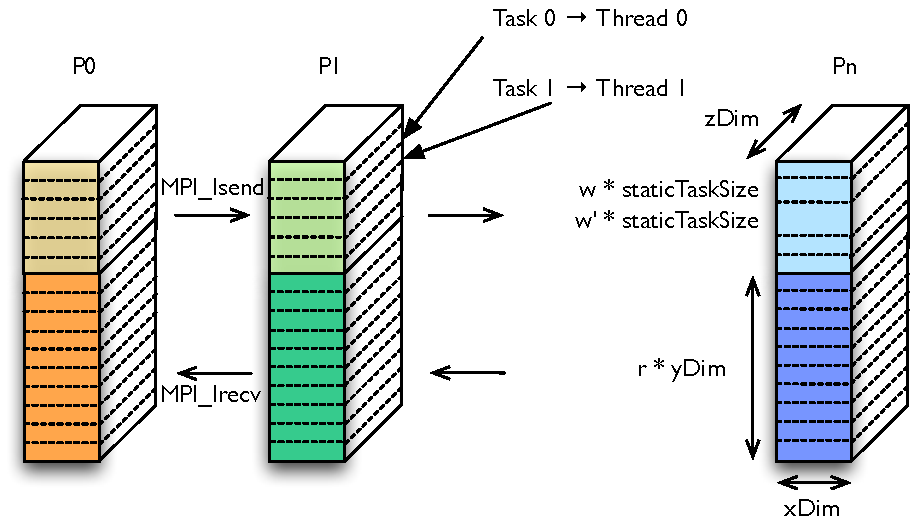
\includegraphics[width=\textwidth]{images/weighted_decomp}
Weighted $\mu$-sched 
\end{columns}
\end{frame} 

\begin{comment}
\begin{frame}
\begin{columns}
\column{0.5\textwidth}
\frametitle{Our Solution}
Original 
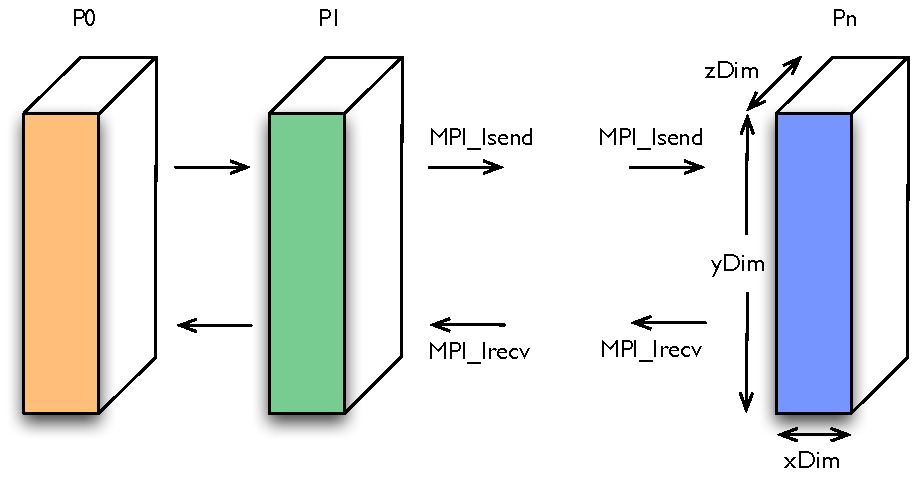
\includegraphics[width=\textwidth]{images/mpi_decomp}
$\mu$-sched 
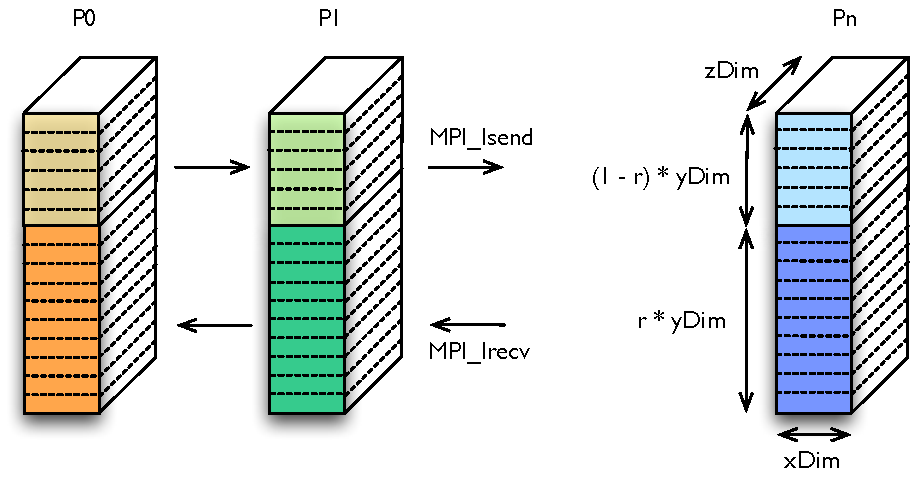
\includegraphics[width=\textwidth]{images/hybrid_decomp}
Weighted $\mu$-sched 
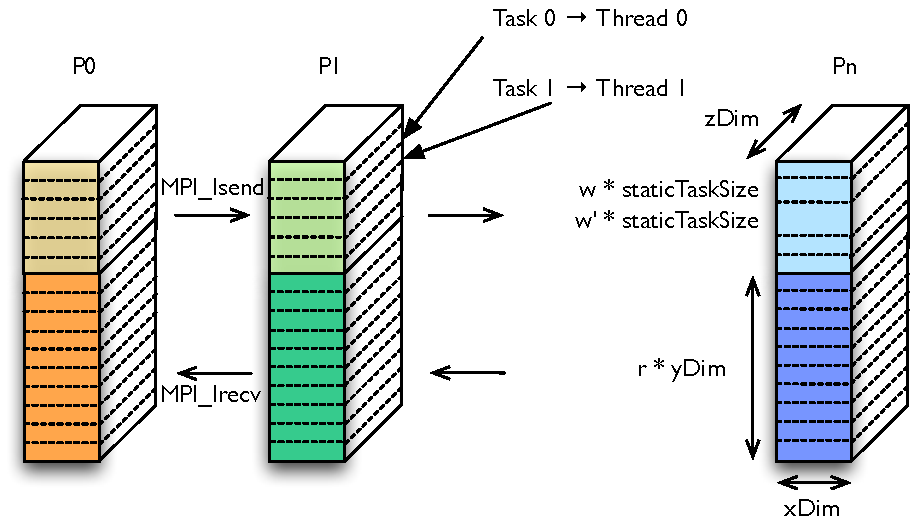
\includegraphics[width=\textwidth]{images/weighted_decomp} 
\column{0.5\textwidth} 

\textbf{Original} \\ \\ \\  

\textbf{$\mu$-scheduling} \\ \\ \\  

\textbf{Weighted $\mu$-scheduling} \\ \\ \\  

\end{columns}
\end{frame} 
\end{comment}

\begin{frame}
\frametitle{Scalability of Different Scheduling Strategies(Jaguar)}
%\begin{block}{}
%Enlosing text in the ``block'' environment
%creates a distinct, headed block of text. 
%\end{block}
%\begin{block}{Scalability of Schedulers}
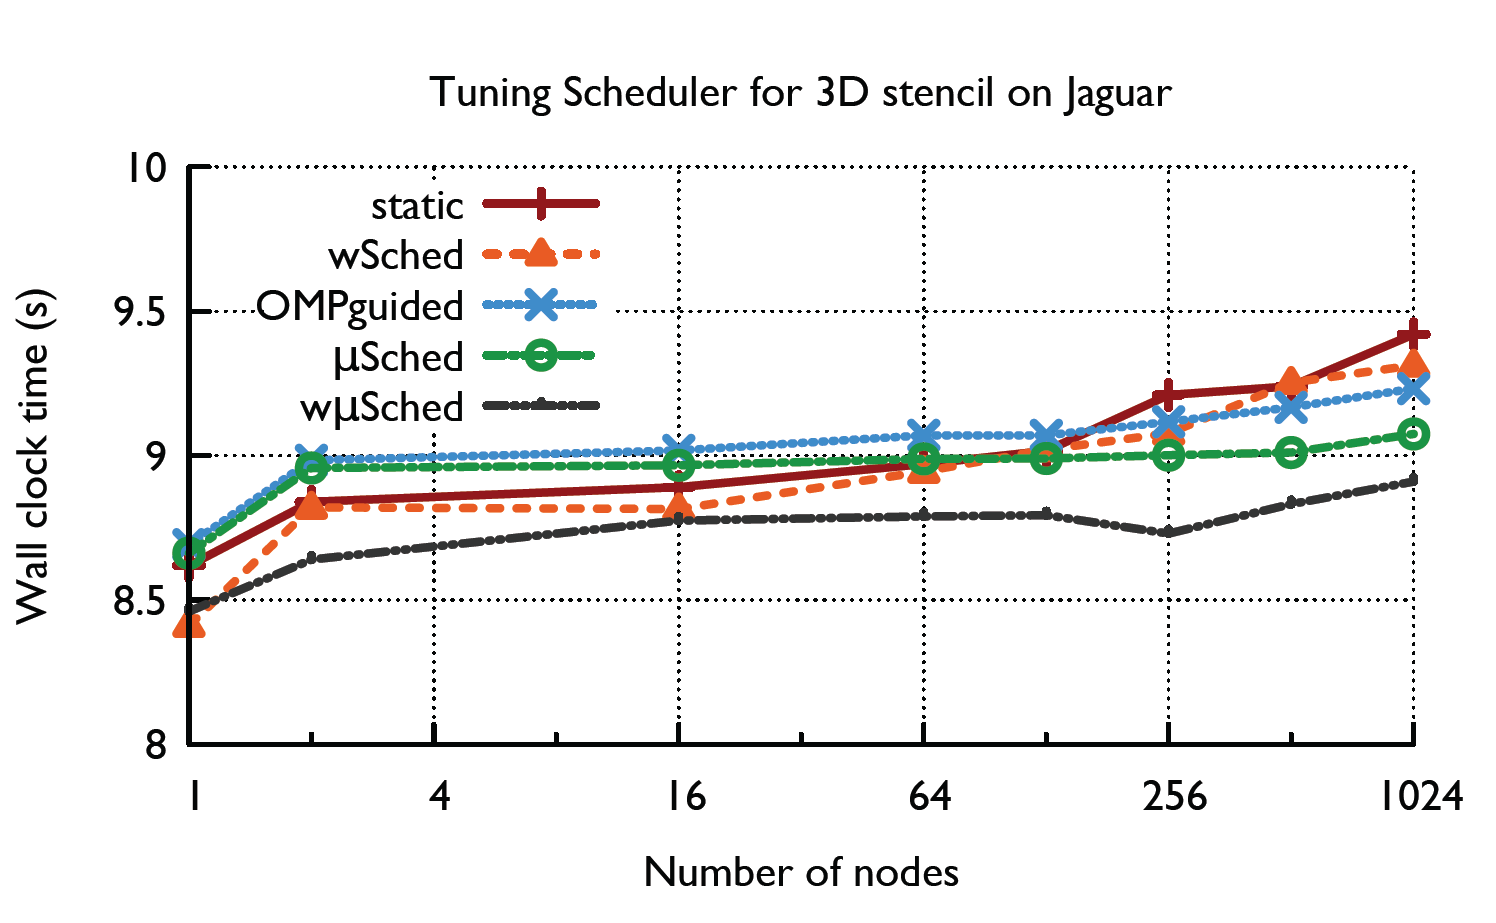
\includegraphics[width=\textwidth]{images/schedulerTuningJaguar}
\end{frame} 

\begin{frame}
\frametitle{Scalability of Different Scheduling Strategies (Ranger)}
%\begin{block}{}
%Enlosing text in the ``block'' environment
%creates a distinct, headed block of text. 
%\end{block}
%\begin{block}{Scalability of Schedulers}
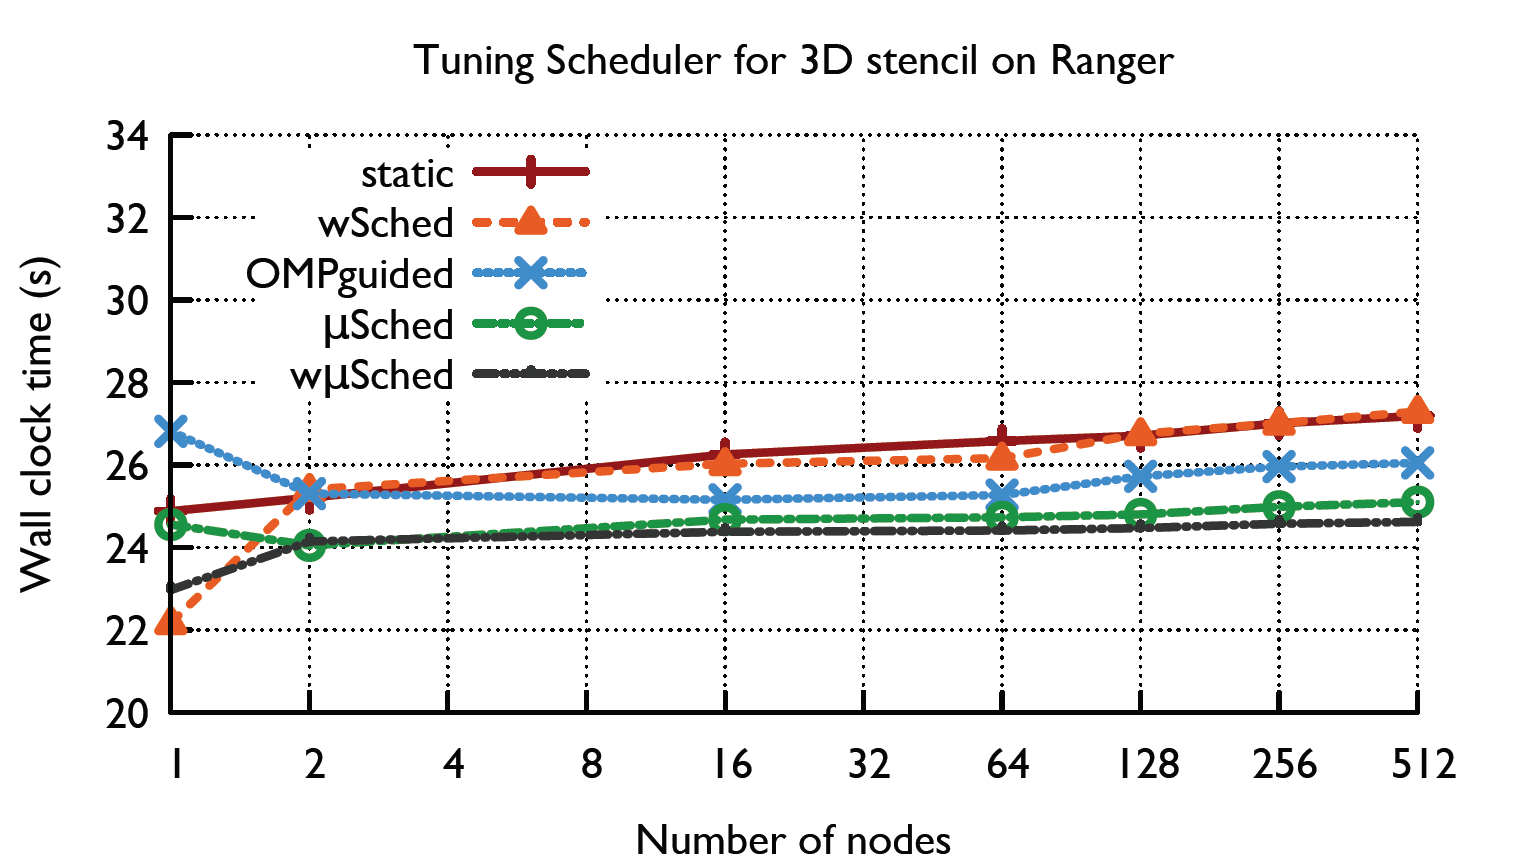
\includegraphics[width=\textwidth]{images/schedulerTuningRanger}
\end{frame}
%\framebox{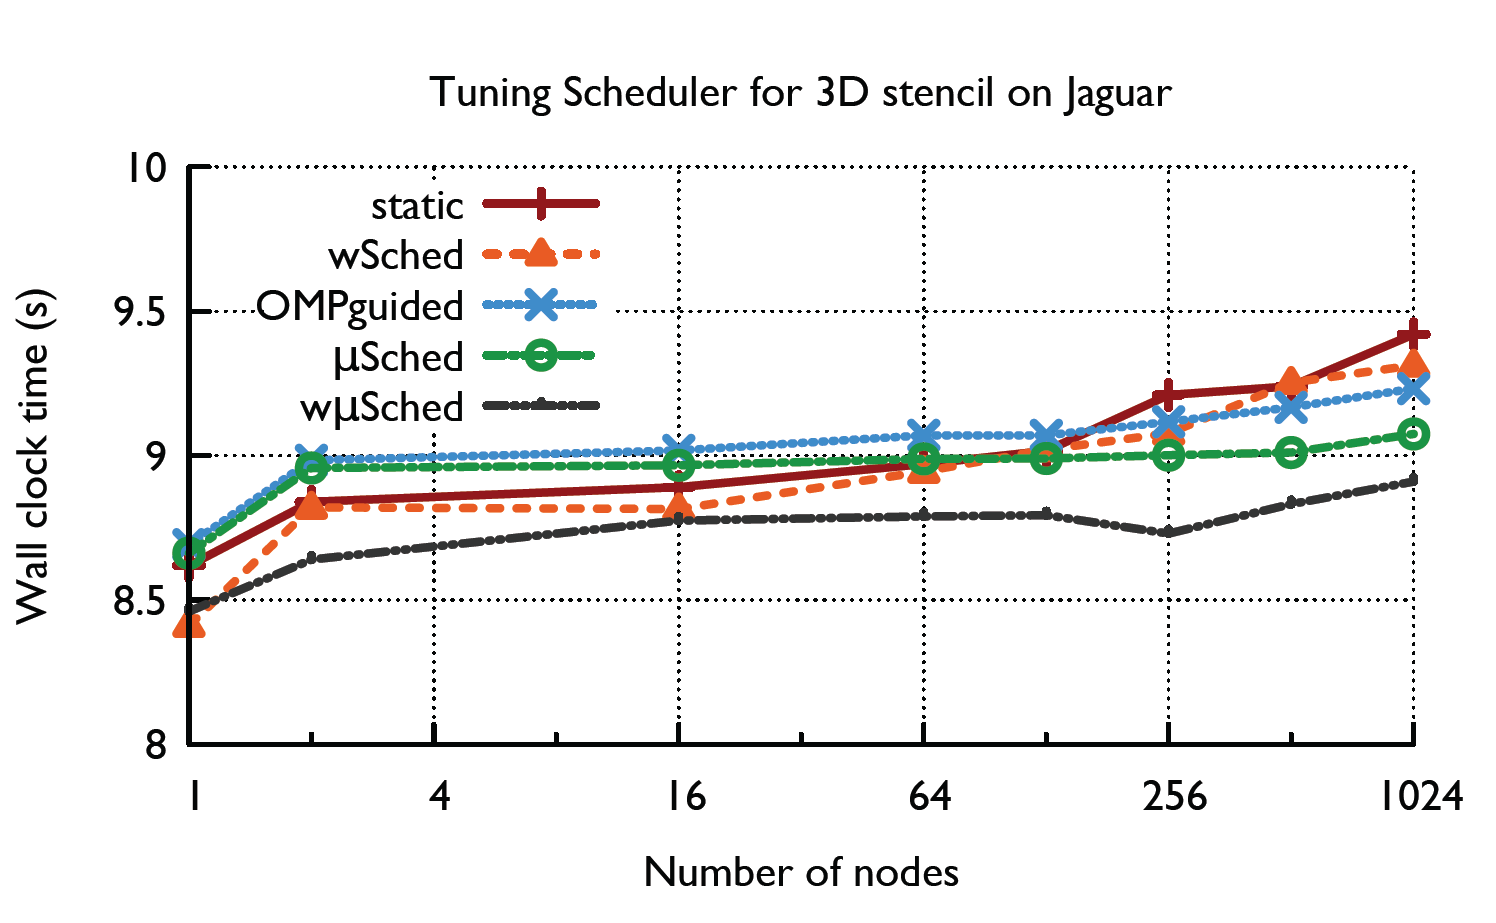
\includegraphics[width=\textwidth]{images/schedulerTuningJaguar}}
%\framebox{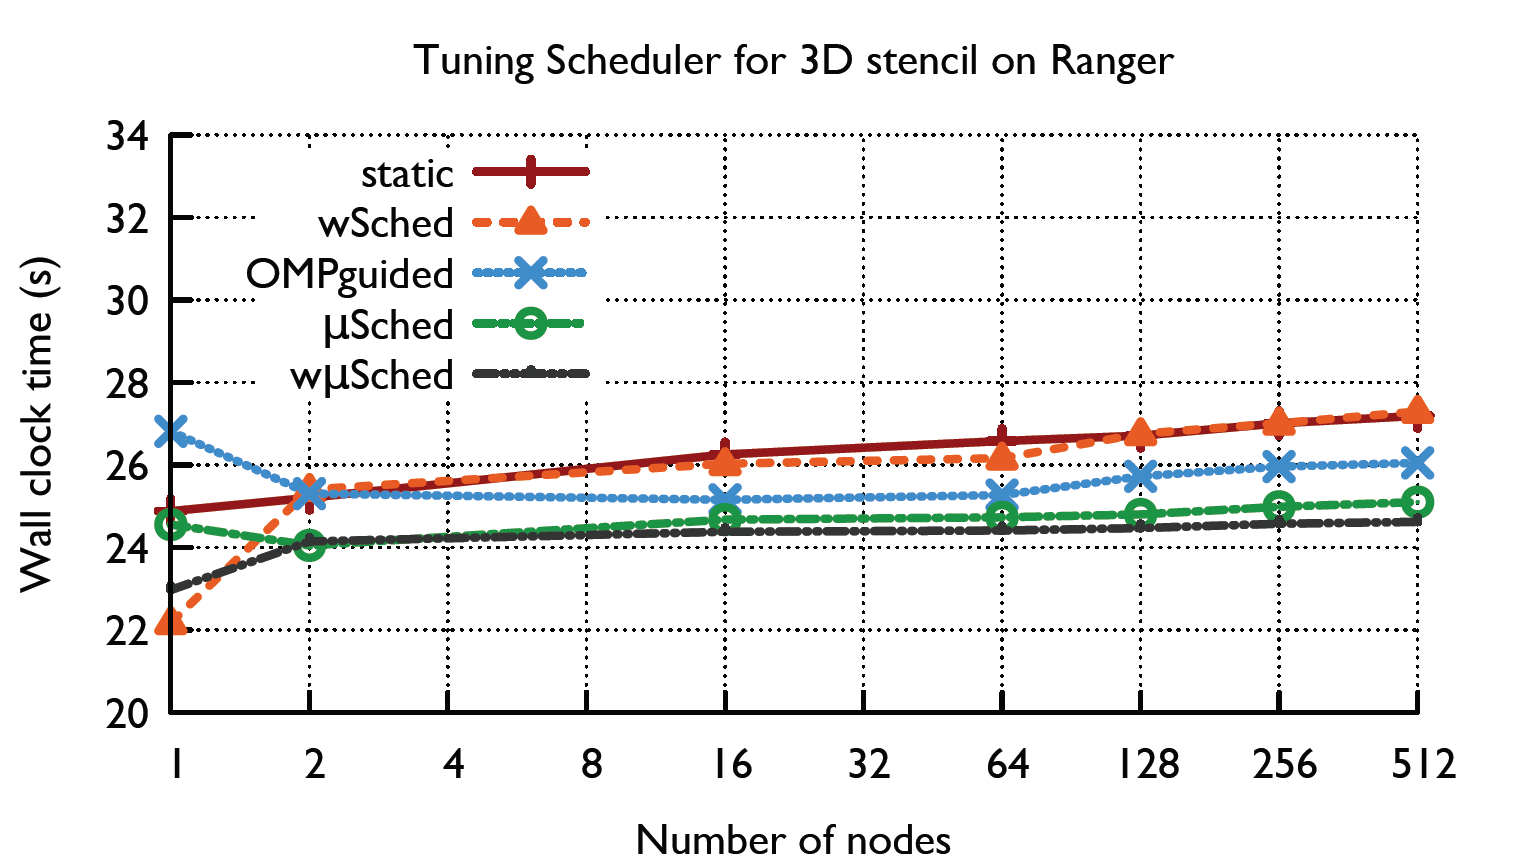
\includegraphics[width=\textwidth]{images/schedulerTuningRanger}}

\begin{frame}
\frametitle{Scalability of Different Scheduling Strategies} 
% \begin{block}{}
% Enlosing text in the ``block'' environment
% creates a distinct, headed block of text. 
% \end{block}
% \begin{block}{Scalability of Schedulers}

\begin{columns} 
\column{0.5\textwidth}
\begin{enumerate} 
\item \tiny Ranger has less dramatic noise amplification inflection
  point; on Jaguar, inflection point at 1024 nodes for static. 
\item \tiny $\mu$-scheduling reduces noise amplification on both machines.
\item \tiny Weighted scheduling gives some improvement on Ranger, and 
significant improvement on Jaguar. 
\item \tiny Weighted $\mu$-scheduling provides noticeable benefits on
  both machines due to new scheduler's ability to handle any mixture
  of low-prob, high-amp load imbalance and high-freq, low-amp load
  imbalance. 
\end{enumerate} 
\column{0.5\textwidth}   
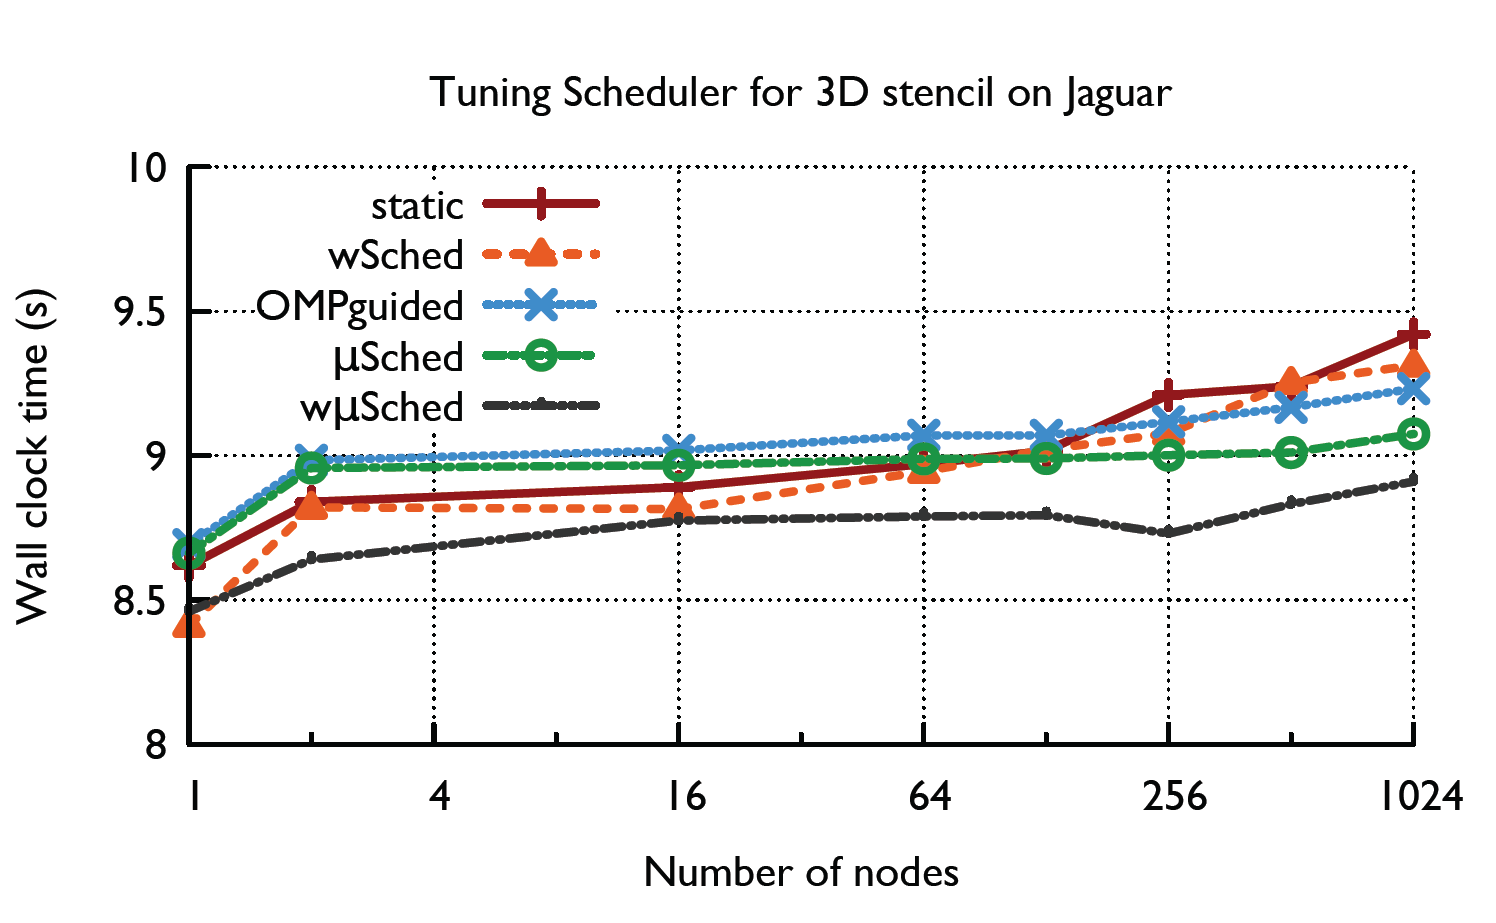
\includegraphics[width=\textwidth]{images/schedulerTuningJaguar}   
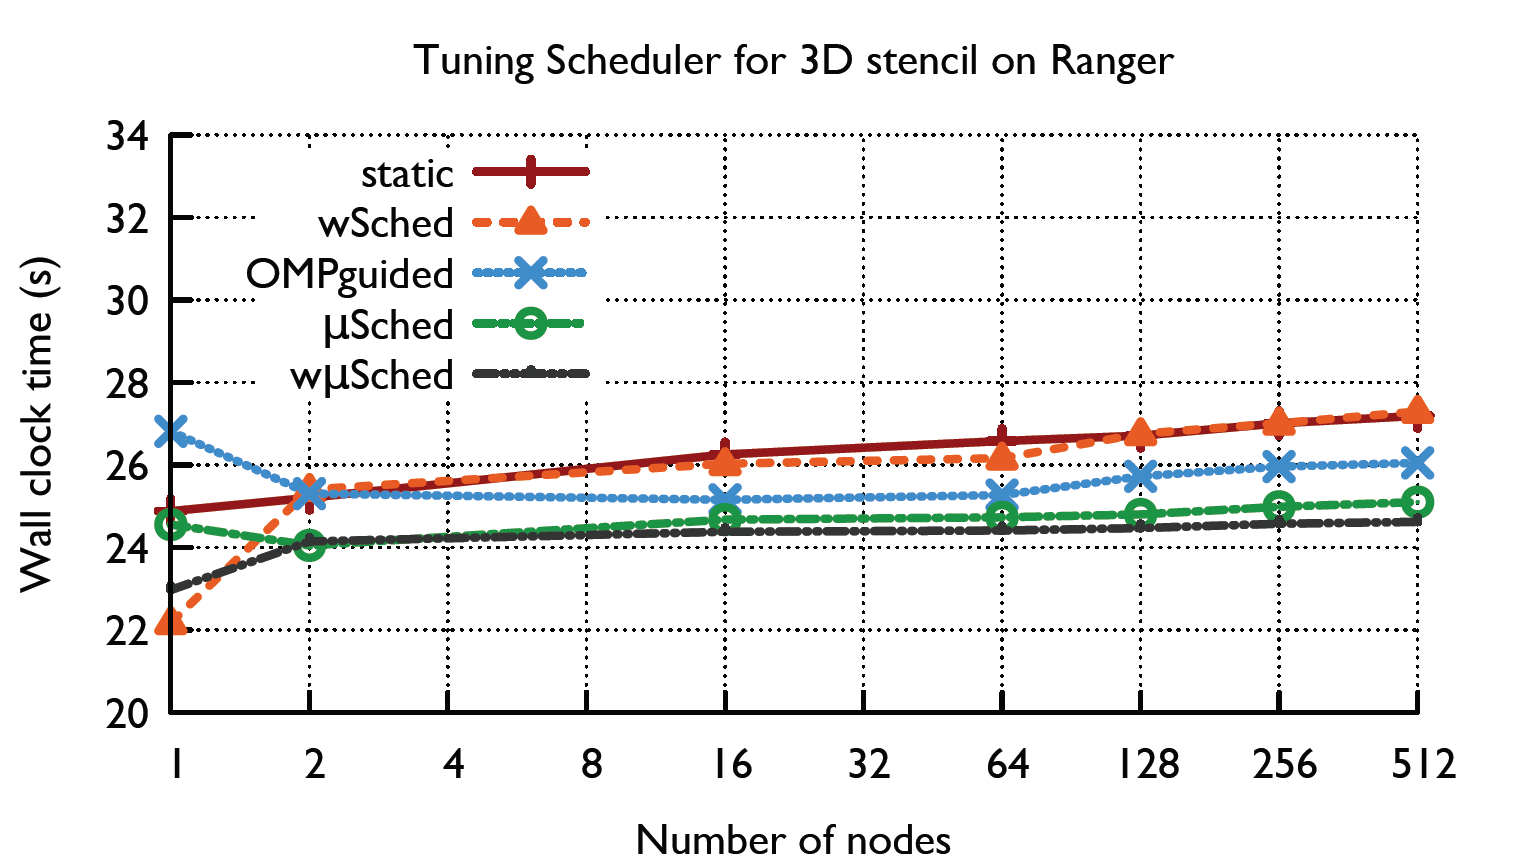
\includegraphics[width=\textwidth]{images/schedulerTuningRanger} 
\end{columns}   
\end{frame} 



\begin{frame}[Two fundamentally different approaches to Load Balancing] 
\frametitle{Two Very Different Approaches to Load Balancing} 
\begin{itemize}
%\item Measurement-based load balancing and work-stealing are two very
%different ways to maximize performance on a machine, based on two very
%different beliefs about parallelism.  
\item Measurement-based load balancing and the work-stealing 
are driven by two different fundamental beliefs about applications and
architectures. 
\item Work-stealing is driven by the belief that computation can be
balanced across processors through the "invisible hand". 
\item Measurement-based load balancing says that computation can be 
balanced through some inferences about the future, given "knowledge" 
and tangible measurements previously. 

\end{itemize} 
\end{frame}  


\begin{frame}[The Second Shortcoming of Pure Work-stealing] 
\frametitle{The Second Shortcoming of Pure Work-stealing}
\begin{itemize}
\item \small Our core work identifies work-stealing as a way to
improve scalability for bulk-synchronous applications. 

\item \small We made the specific point that work-stealing
needs to be ``lightweight'' due to its non-neglible coherence cache
misses and dequeue overheads. \\

\item \small \textit{Second} shortcoming (not thought of in our
prior work): inability to take advantage of the persistent patterns in
noise signatures. \\

\item \small We do find such patterns in noise signatures on many machines 
(two tested in detail were Jaguar and Ranger). \\

%\item \small Several of these high-frequency low amplitude noise events do actually have some defined pattern of load imbalance, specifically targetting a
%particular core.  
\item \small This type of noise is so fine-grained that it makes
it seem as if a particular core is "slower" throughout the duration of 
the timestep. 
\end{itemize}
\end{frame} 

\begin{frame}[Impact of Amount of Computation done in  Application Timestep]
  \frametitle{Impact of Application Timestep Length (Jaguar)}
  \framebox{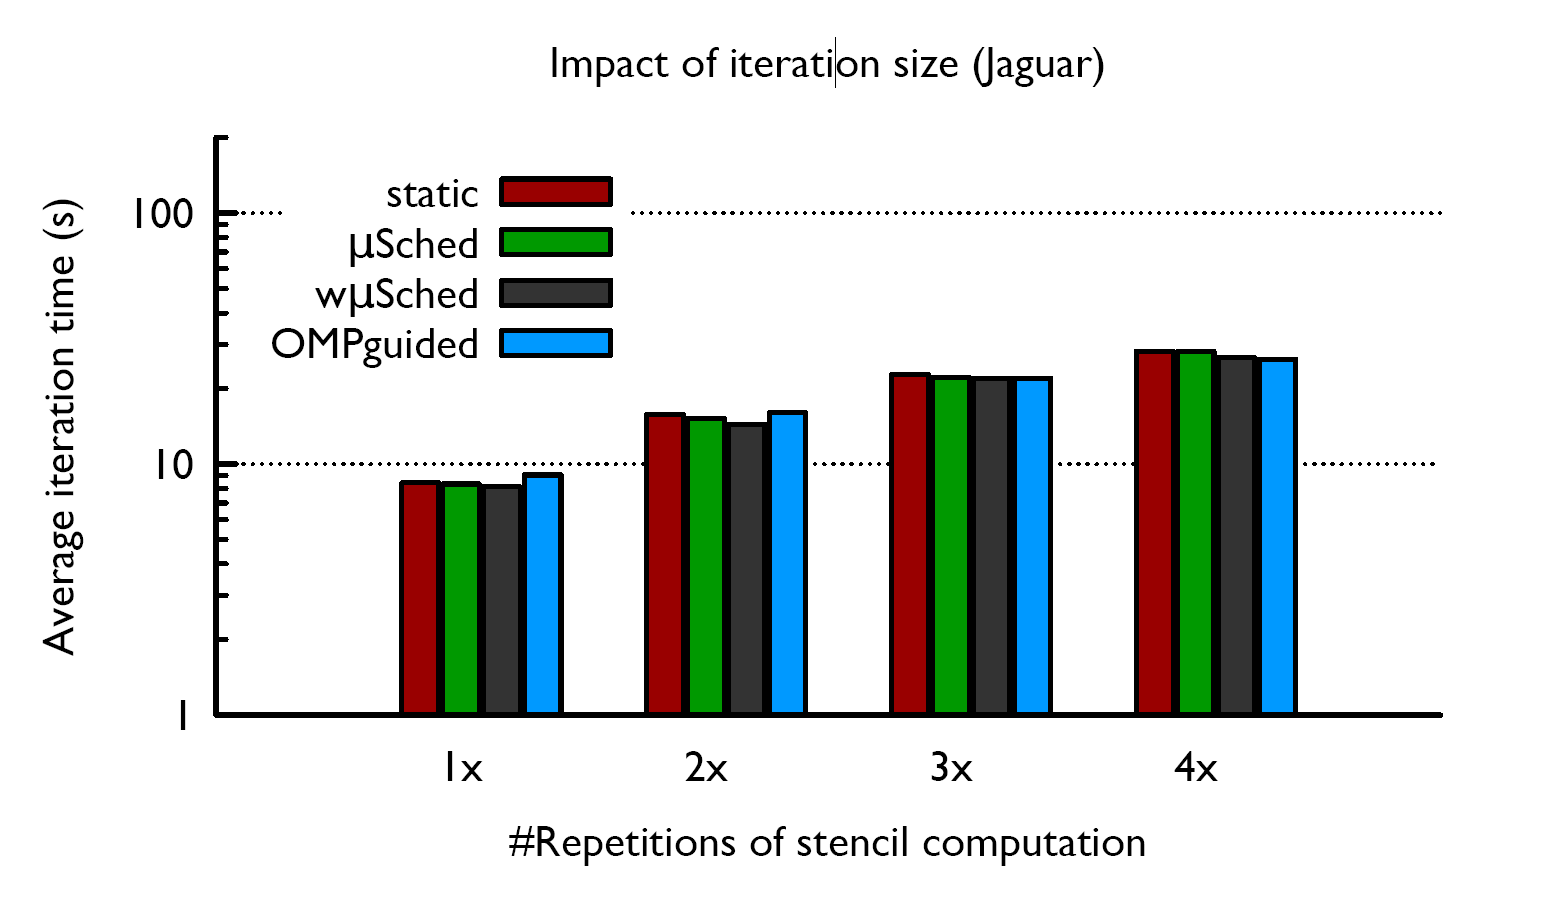
\includegraphics[width=\textwidth]{images/iterSizeImpact-Jaguar}}
\end{frame} 

\begin{frame}[Impact of Amount of Computation done in  Application Timestep]
\frametitle{Impact of Application Timestep Length (Ranger)}
\framebox{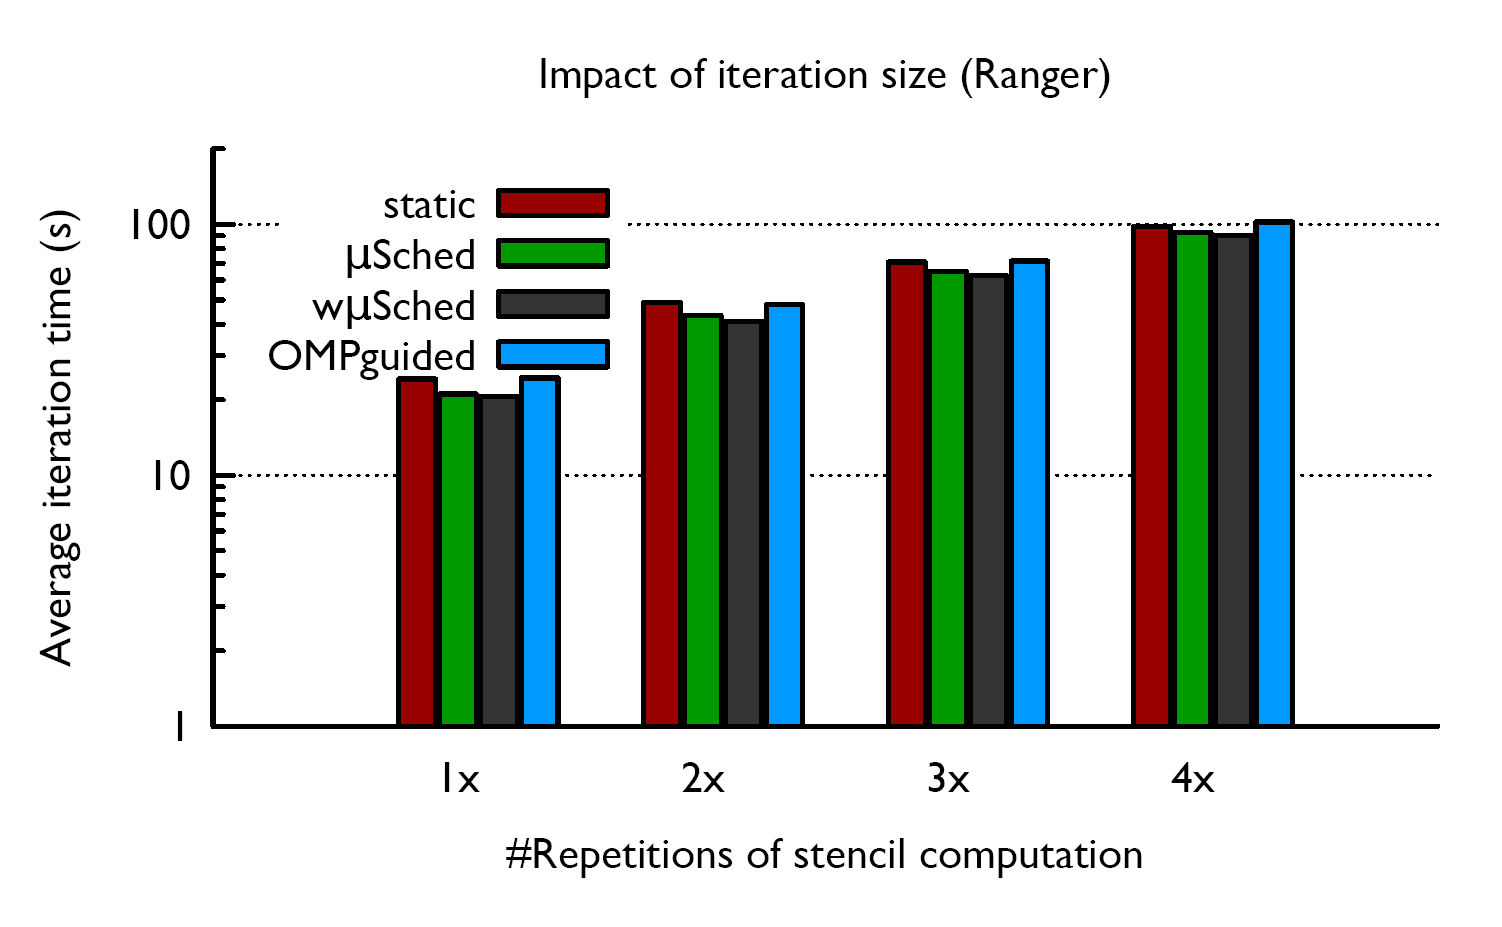
\includegraphics[width=\textwidth]{images/iterSizeImpact-Ranger}}
\end{frame} 

\begin{frame}[Impact of Amount of Computation done in Application Timestep]
\frametitle{Impact of Application Timestep Length}
\begin{columns}
\column{0.5\textwidth}
\begin{enumerate}
\tiny \item \tiny For baseline static scheduling, an application with larger time steps
seems to suffer less from system noise. 
\item \tiny For Jaguar, $\mu$-scheduling is worse than guided
  scheduling for large timesteps. 
\item \tiny For both machines, our strategies are competitive with and seem to perform
  better than the standard OpenMP guided scheduling, regardles of  app
  timestep length.  % p1 app-iterSize 
% \item overall impact of noise on load imbalance increases 
% linearly with the amount of computation done per time step,
% particularly for Jaguar. 
% p2 app-iterSize 
%\item \small      % p3 app-iterSize 
\end{enumerate} 
\column{0.5\textwidth}
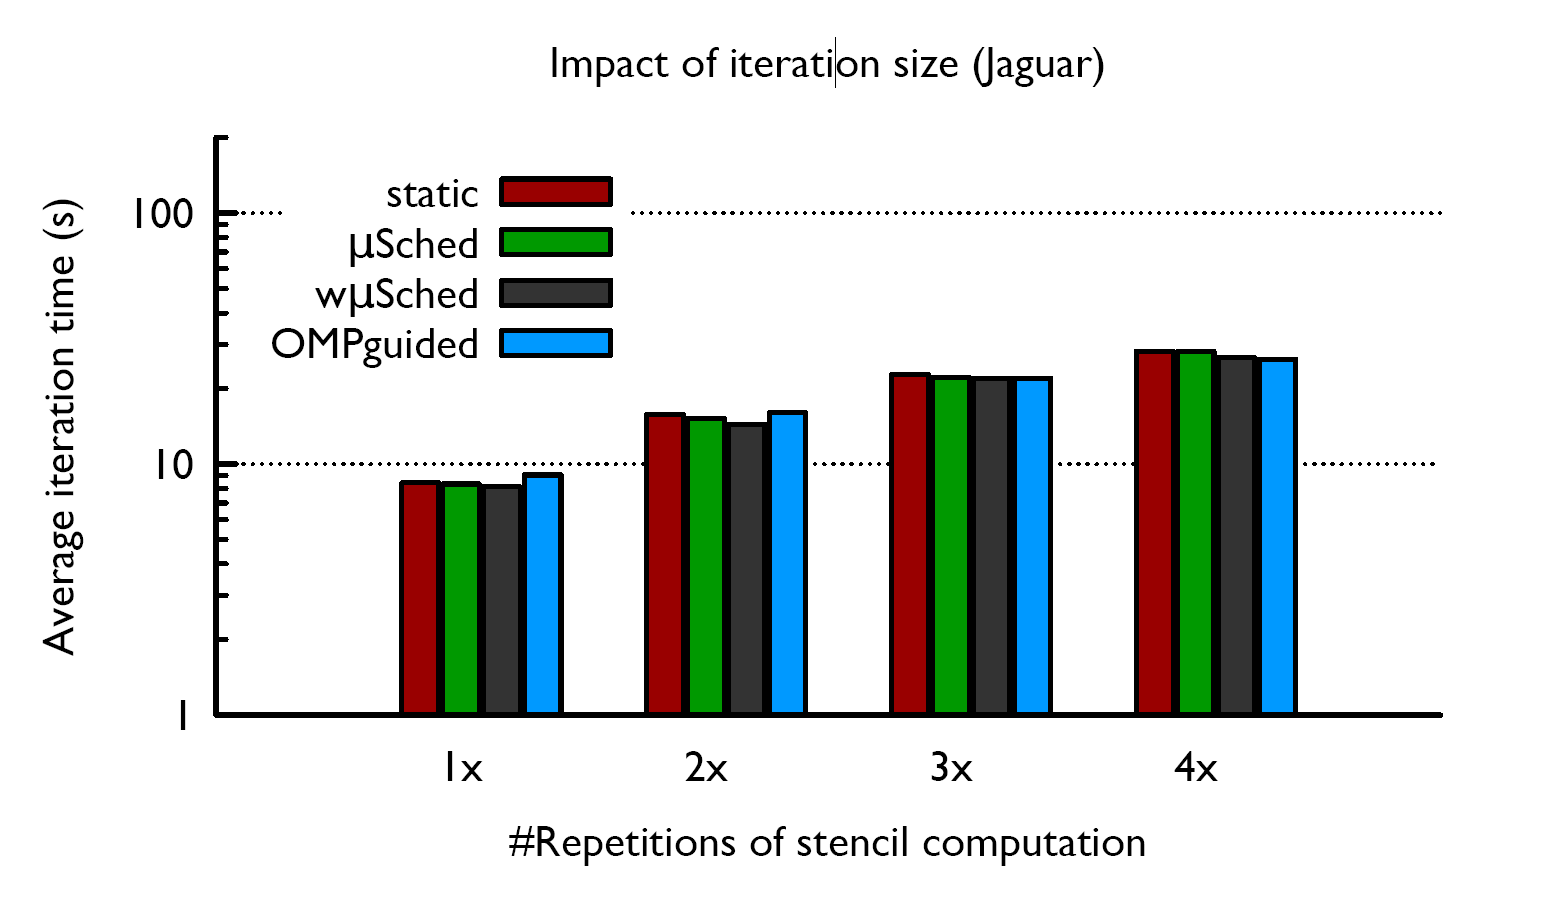
\includegraphics[width=\textwidth]{images/iterSizeImpact-Jaguar}
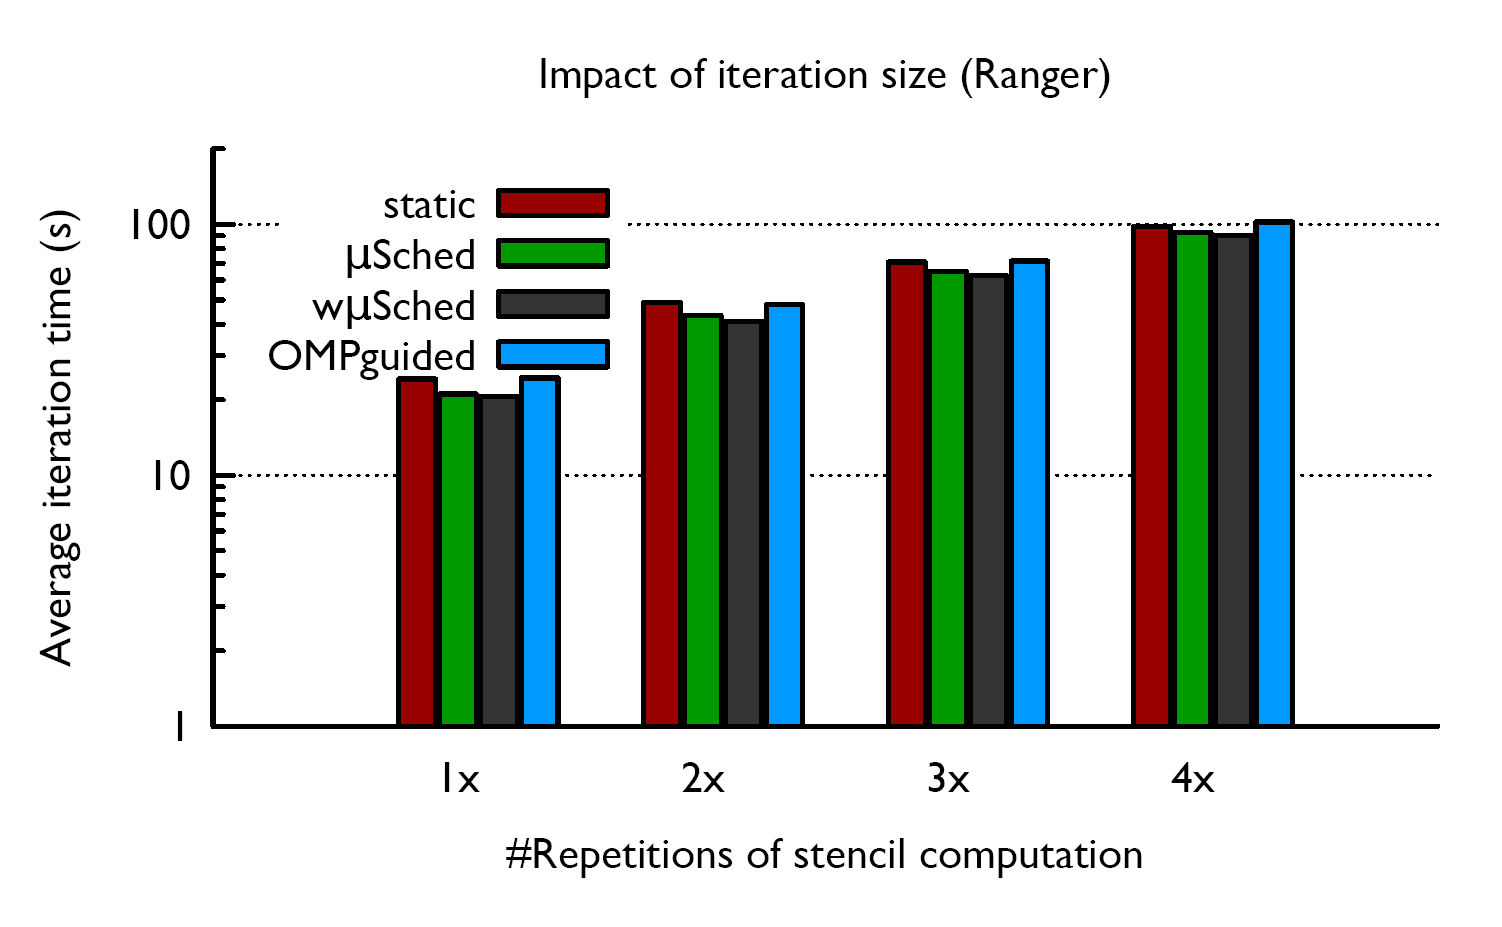
\includegraphics[width=\textwidth]{images/iterSizeImpact-Ranger}
\end{columns} 
\end{frame} 

\begin{frame}[Impact of Problem Size] 
\frametitle{Impact of Problem Size (Jaguar)} 
\framebox{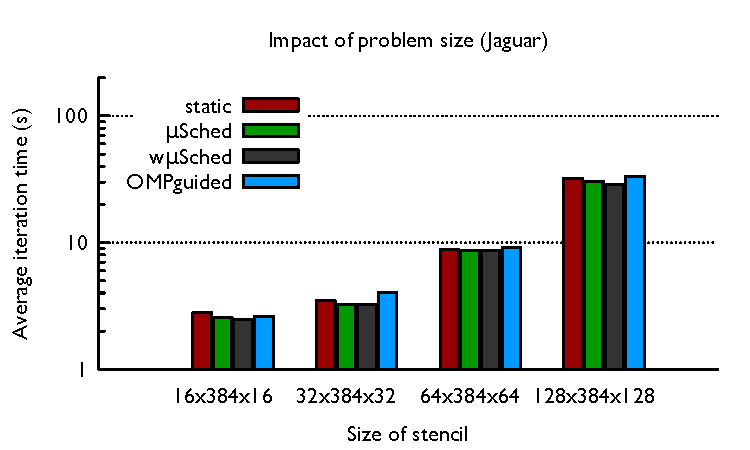
\includegraphics[width=\textwidth]{images/probsize_jaguar}}
\end{frame} 

\begin{frame}[Impact of Problem Size]
\frametitle{Impact of Problem Size (Ranger)}
\framebox{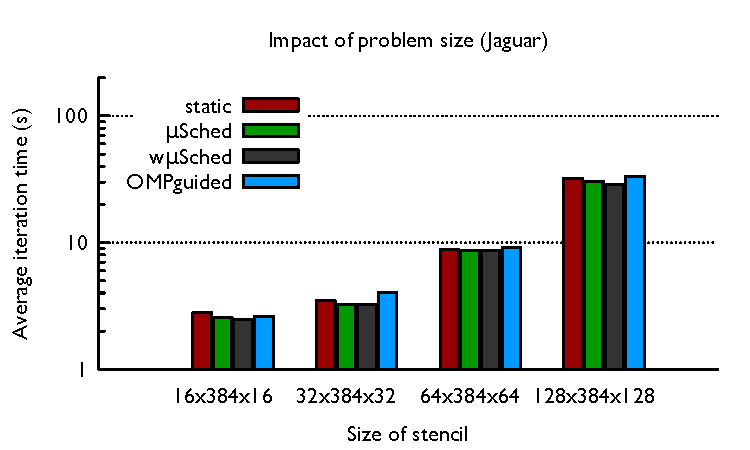
\includegraphics[width=\textwidth]{images/probsize_ranger}}
\end{frame} 

\begin{frame}[Impact of Problem Size]
\frametitle{Impact of Problem Size}
\begin{columns}
\column{0.5\textwidth}
\begin{enumerate}
\tiny \item \tiny For small problem sizes, any delay is more likely than
not due to system noise, and not latency of access to off-chip cache
or main memory. 

% p1 app-probSize
\item \tiny The lack of bene????t for larger problem sizes on both
  Jaguar and Ranger is likely due to the fact
that performance is already impacted by memory bandwidth
limitation.  % p2 app-probSize
\item \tiny Note that memory bandwidth limitation should not be
  confused with noise, but that the weighted scheduling could actually serve
to reduce impact of mem bandwidth strain particularly if shared mem access
is non-uniform. 
% p3 app-probSize
\end{enumerate} 

\column{0.5\textwidth}
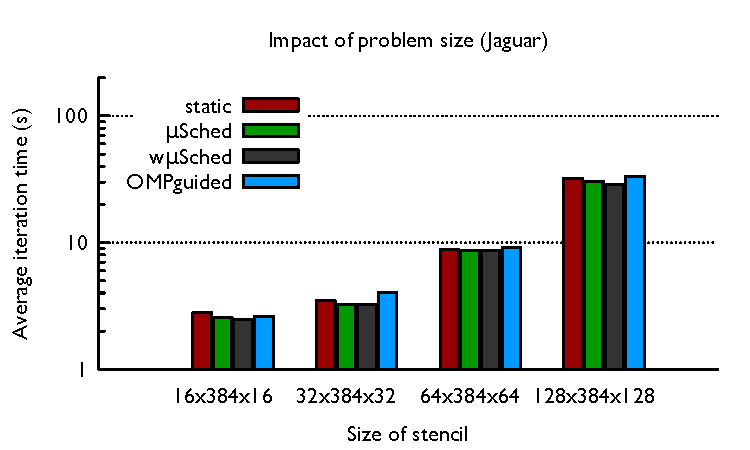
\includegraphics[width=\textwidth]{images/probsize_jaguar}
\includegraphics[width=\textwidth]{images/probsize_ranger}
\end{columns}
\end{frame} 
 
\begin{frame}[Discussion]
\frametitle{Discussion} 
\begin{itemize}
\item \small Architectures may advance yearly, but remember that OS is changing and advancing also.
\item \small Operating system may have been programmed 
inefficiently, creating larger overheads than 
one would expect. The net effect of inefficient
programming of Operating System is again more OS noise. 
\item \small  The ``noise'' \textit{does not just come from the OS}; it 
can also come from hardware variations, app load imbalance, runtime, 
interaction between app and runtime, hybridized runtimes, ... \\  
\item \small To statically parallelize the entire
hardware/software stack is very difficult, and so an adaptive, lightweight scheduling
seems to be the right solution to scale past the noise amplification problem
(and works with good success, as our results show). 
\end{itemize}
\end{frame}  



\begin{frame}[Conclusion]
\frametitle{Conclusion}
\begin{itemize}

\item \small  Two different types of load imbalances: 1.  high-frequency,
  low-amplitude, asymmetric and 2. low-probability,
  high-amplitude, symmetric.

%\item  \tiny For these two load balancing schemes, there are two
%  different types of load balancers: load
%  balancing across application timesteps (measurement-based load
%  balancing) and load balancing within an application
%  timestep (work-stealing). 

\item \small Jaguar has more type 1 load imbalances than Ranger. It has
  less of type 2 load imbalances.  Ranger has less of type 1, 
  though type 2 still exists. \\

\item \small By incorporating a weighted scheduling scheme with 
our original $\mu$-scheduler, we can handle these two types of load imbalances
  together. \\

\item \small Our results continue to mitigate the noise amplification
  problem, while further bringing down the constant factor loss in
  performance due to task quantization that would otherwise occur with 
our lightweight scheduling. \\
 
\item \small Our load balancing scheme provides more performance benefit
on Jaguar due to a larger amount of the asymmetric, high-frequency,
low amplitude load imbalances. \\ 

\end{itemize}
\end{frame}

\begin{frame}   
\frametitle{Future Work} 
\begin{itemize}
\item Implement and integrate into numerical linear algebra library. 
\item Look into modifications to periodic load balancer
of measurement-based load balancers 
to try to handle high-frequency, low-amplitude noise events. 
\item See if this could actually also give
some benefit for particle simulations. 
%\item  Consider implementation of using 
%Charm load balancing framework. 
\end{itemize}
\end{frame}

\begin{frame}[Thank You!]
\frametitle{Thank You!}
\end{frame}

\begin{frame}[Related Work]
\frametitle{Related Work}
\begin{enumerate}

\item Work-stealing with Trim Analysis 
\item PLASMA and DPLASMA 
\item Zoltan load balancing 
\item Charm load balancing
\item Co-scheduling
\item FASTOS
\item Tesselation 

\end{enumerate} 
\end{frame}

\begin{frame} 
\frametitle{What the Plots Can Tell Us}


\begin{itemize}
\item \small Frequency plot tells us about amplitude of noise events,
  and the number of distinct noise event lengths. Low-amplitude noise events
  implies fine-grained load imbalance. \\ 

\item \small Noise spread tells us about the distribution of noise
  across cores. Low, well-defined bands tells us that some cores suffer
  high-frequency, low-amplitude and \textit{asymmetric} load
  imbalance. \\ 

\item \small Noise time series plot tells us about persistency in load
  imbalance. \\ 

% The periodicities can be seen by the even spread of noise
%  across time. 

\end{itemize}
\end{frame} 


\begin{frame}
\frametitle{Noise Characterization for Jaguar and Ranger}
\begin{itemize}
\item \small Ranger's noise plot has some high-frequency low-amplitude
  noise, but has more of the low-probability, high-amplitude noise
  events.  
% though the asymmetry is not defined. 
\item \small Jaguar's noise signatures have both low-probability,
high-amplitude noise events and  high-frequency, low-amplitude 
noise events on some particular cores. 
\item \small Distribution of noise across cores seems to be somewhat
random for Ranger, but more well-defined for Jaguar. 
%\item \small This high-frequency, low-amplitude noise is
%\textit{across multiple timesteps},
\item \small This results in different balance of high-frequency,
  low-amplitude noise events and low-probability, high-amplitude noise
  events on each of the machines. 
\end{itemize}
\end{frame}

%\begin{frame}
%\frametitle{Acknowledgements}

%\begin{itemize}
%\item .
%\item Maria Garzaran
%\item Laxmikant Kale 
%\item Franck Cappello 
%\end{itemize}
%\end{frame}






\begin{frame}[Theoretical Analysis]
\frametitle{Theoretical Analysis of Lightweight Scheduling}
\begin{itemize}
\item \tiny Let $t = T_p$ be the time for each phase when $p$ processing elements
work together, in absense of noise (and assuming fully static scheduling). \\
\item \tiny Let $T_{p}'$ be the time for each phase, in the presence of noise, along with scheduler overhead needed
to counter/mitigate this noise. \\
\item \tiny Let $\delta_{max}$ be the duration of the longest length noise event. \\
Let $\delta_{avg}$ be the average duration across all noise events.  \\
We do \textit{not} assume in this analysis that the length of the noise event is fixed. \\
\item \tiny Let $\phi$ be the probability that noise events happen during a
particular phase on some core. We assume that the probability is the same
across each phase. Furthermore, we assume that the noise event occurs 
(W.L.O.G.) on core 0. \\ 
% consider a Pareto distribution. 
\item \tiny Let $f_{s}$ be the fraction of work scheduled statically. \\
\item \tiny Let $\tau$ be the duration of each dynamic task. \\
\item \tiny $d$ is the average number of dynamic tasks enqueued by each
processing element (in a perfectly load balanced iteration). \\
\item \tiny Let ${t_q}(p)$ be the dequeue time for pulling work from one's
own pile. In general, this dequeue time may depend on the number of processing
elements. \\ 
%\item Let $\Gamma$ be the time needed to move one task from one
%processing element's queue to another processing element's queue. This
%is effectively the cost of a coherence cache miss. \\
%\item Let W be the total number of FLOPS to be done by all $c$
%cores.
\end{itemize}
\end{frame} 

\begin{frame}[Theoretical Analysis: Static Fraction Bound]
\frametitle{Theoretical Analysis: Static Fraction Bound}

What is the percentage of dynamic scheduling that we need, before the
cost of the lightweight scheduler's scheduling overhead outweighs its
benefit of ``noise'' mitigation (i.e. parallelization of unpredictable
excess work inducing transient load balance)? \\

\textbf{Theorem 1:} \\
 $f_{s} \leq 1 - \frac{{\delta}_{max} -{\delta}_{avg}}{T_{p}}$ \\ 
\end{frame} 

\begin{frame}[Theoretical Analysis: Expected Time for Application Timestep]
\frametitle{Theoretical Analysis: Expected Time for Application Timestep}

What is the expected time necessary for one application timestep to
complete, given some characterization of noise, pre-tuned static
fraction(from above), and known scheduler overheads(which are platform
dependent)?  Here, let us assume that $\delta$ = $\delta_{max} -
\delta_{avg} $. \\

\textbf{Theorem 2:} \\ 
 $ T_{p}' = (1 - {\phi}){\Pi}_0 + (\phi)((\frac{T_p -\delta}{T_p}){\Pi}_1 + (\frac{\delta}{T_p}){\Pi}_2) $ \\ 

where \\  
${\Pi}_0$ = $T_p + d \cdot {t_q}(p)$ \\  
${\Pi}_1 = {\Pi}_0 + (\tau + {t_q}(p) + \Gamma) \lceil \frac{\delta}{\tau \cdot p} \rceil $ \\
${\Pi}_2$ =  $T_p + \epsilon + (d - \lfloor \frac{\delta - \epsilon}{\tau + {t_q}(p)} \rfloor) \cdot {t_q}(p)$ \\ 

\end{frame}  


\begin{frame} 
\frametitle{Research Question} 
\begin{itemize} 
\item \small Can we improve full-scale run of PF3D and MILC through using
 global information to build a generalized lightweight scheduler that
 avoids scheduling on those nodes not on critical path of dependences
in MPI communication? 

\item \small What can we do to improve full-scale run of PF3D and 
MILC through using global information to build a generalized
lightweight scheduler that avoids scheduling on those nodes not on
critical path of dependences in MPI communication? 

\item \small How can we improve scalability of PF3D and 
MILC through using global information to build a generalized
lightweight scheduler that avoids scheduling on those nodes not on
critical path of dependences in MPI communication? 
\end{itemize}

\end{frame}


\begin{frame}
\frametitle{Slack Concscious Scheduling}
\begin{itemize}
\item Baseline slack evolution
\item Slack variation histogram  
\item Average Slack per Process (which process is on the critical path?)
\end{itemize}
\end{frame}

\begin{frame}
\frametitle{Experimentation of slack-conscious lightweight scheduling:
  PF3D/MILC} 
\begin{itemize}
\item num Processes vs wall clock time 
\item Histogram analysis
\end{itemize}  
\end{frame}  


\begin{frame}
\frametitle{Simulation of slack-conscious lightweight scheduling
through PF3D} 
\begin{itemize}
\item 1
\item 2 
\item 3
\end{itemize}
\end{frame}


%\begin{frame}[Traditional Data Parallelism]
%\frametitle{Core Problem Statement}
%\begin{itemize}  
%\item We can take advantage of the parallelization by trying to do a
%  perfect domain decomposition and splitting work evenly across
%  threads. 
%\item The assumption here is that all the processing elements will be
%  used all the time. 
%\end{itemize}
%\end{frame}

%\begin{frame}[Many Different Solutions]
%\frametitle{Separate Research Questions for Jitter Mitigation}
%  \begin{figure}
%    \includegraphics[width=0.65\textwidth]{JitterMitigationSolutionStack}
%  \end{figure}
%  \includegraphics[width=0.65\textwidth] 
%\end{frame}

%\begin{frame}[Separate Solutions]
%\frametitle{Separate Solutions}
%  \begin{itemize} 
%  \item \textit{Application-level:} 
%    \begin{itemize}
%    \item using auto-tuned micro-scheduling
%    \item abstractions for tuning micro-scheduling
%    \end{itemize} 
%  \item \textit{Runtime-level:} 
%    \begin{itemize}
%    \item Can use online machine learning to assess performance
%    variation and tune accordingly at runtime.
%    \item Could develop (or extend) an ``intelligent'' runtime system
%    that automatically handles noise mitigation behind the scenes,
%    detecting patterns in noise load imbalance through measurements
%    taken at runtime. 
%    \end{itemize}


%  \item \textit{System-level:}
%    \begin{itemize}
%    \item co-scheduling and gang-scheduling 
%    \item process migration
%    \end{itemize}


%  \item \textit{Platform-level:}
%    \begin{itemize}
%    \item Judiciously stripping away OS services
%    \item Creating abstractions to strip away such services
%    \end{itemize}
%  \end{itemize}
%\end{frame}
 
%\section{Coding} 
%\begin{frame}
\frametitle{Coding Table of Contents}
\tableofcontents[part=1]
\end{frame} 

\subsection{Scheduler Runtime}
\subsubsection{Scheduler Runtime: Must have} 
\begin{frame}
\frametitle{$\mu$-Scheduler runtime: Must Have}
\begin{enumerate} 
\bllt \sout{create interface}
\bllt Consider usage in context of MPI shared memory extensions.
\bllt Testing infrastructure for correctness. 
\begin{itemize} 
\item \tiny Check answer of Dot Product. Can use norms. 
\item \tiny Check all threads are running and doing work. 
\item \tiny Check for lock and unlock (no data races). 
\item \tiny Check total work done, regardless of sched. (no tasks should be left behind) 
\item \tiny Check locality state info is getting updated. 
\end{itemize}
\bllt Incorporate state information in scheduler. 
\begin{itemize}
\item \tiny Add integrate MPI slack-conscious sched. 
\item \tiny Add in thread slack-conscious sched. 
\item \tiny Add in tasklet locality tags. 
\end{itemize}
\end{enumerate} 
\end{frame} 

\subsubsection{Sched Runtime Should have}
\begin{frame}
\frametitle{Sched Runtime: Should Have}
\begin{enumerate} 
\bllt Create separate files for schedulers(?). 
\bllt See if we can get an OpenMP like interface. 
\bllt make proper output, and redirect to file. 
\bllt use gnuplot scripts to get data from output file. 
\bllt package into ar and shared library. 
\end{enumerate}
\end{frame}

\subsubsection{Sched Runtime : Nice to have}
\begin{frame}
\frametitle{Sched Runtime: Nice to have}
\begin{enumerate} 
\bllt put in proper timers for slack-conscious scheduling
\bllt get profiling to measure dequeue overhead 
\end{enumerate} 
\end{frame} 

\subsubsection{Post-processing data}
\begin{frame}
\frametitle{Plotting data}
\begin{enumerate} 
\bllt Plotting for num processes versus perf 
\bllt Transpose
\bllt Runtime overheads for different tuned versions
\bllt output parsing scripts 
\end{enumerate} 
\end{frame} 

\begin{frame}
\frametitle{Output post-processing}
\begin{enumerate} 
\bllt Memorize the code needed for file I/O. Consider C++ file I/O. 
\bllt Have a standard table for printing the output through a set of parameters.
\bllt Learn python to post-process the output from an application. 
\end{enumerate} 
\end{frame} 

\begin{frame}
\frametitle{Plotting}
\begin{enumerate} 
\bllt Understand how to create a histogram 
\bllt Know how to label axes and graph title. 
\end{enumerate} 
\end{frame} 

\subsubsection{Git Repo}
\begin{frame}
\frametitle{Git Repo}
\begin{enumerate} 
\bllt Make sure everything compiles before checking in. 
\bllt Check how to do branches in git. 
\bllt Do frequent check-ins. 
\bllt Know what to do in the event of a conflict. 
\end{enumerate} 
\end{frame} 

\subsubsection{Git Repo}
\begin{frame}
\frametitle{Git Repo}
\begin{enumerate} 
\bllt Make sure everything compiles before checking in. 
\bllt Check how to do branches in git. 
\bllt Do frequent check-ins. 
\bllt Know what to do in the event of a conflict. 
\end{enumerate} 
\end{frame} 

\subsubsection{SSH login guide}
\begin{frame}
\frametitle{SSH login guide}
\begin{enumerate} 
\bllt Fix \texttt{known\_hosts} if login creates a problem. 
\bllt Make sure there is an easy way to login without the RSA key.
\end{enumerate} 
\end{frame} 

\subsubsection{Benchmark tests}
\begin{frame}
\frametitle{Tests}
\begin{enumerate} 
\bllt Benchmark tests for load imbalance across cores \texttt{ld} is the linker.
\bllt test for variation across Iteration timesteps
\bllt test for variation across different MPI procs 
\bllt test for variation of dequeue overheads, for one particular thread. 
\bllt test for non-uniformity of dequeue overhead, across threads. 
\end{enumerate} 
\end{frame} 

\subsubsection{Work Improvement}
\begin{frame}
\frametitle{ }
\begin{enumerate} 
\bllt Send email on tasks/habits on Monday
\bllt Add tasks in JIRA 
\bllt finish cases for theoretical analysis + send this out
\bllt finish writing of theoretical analysis. 
\end{enumerate} 
\end{frame} 

%\section{Thesis Notes}
%\begin{frame}[Problems] 
\frametitle{Context for CSE}
\begin{enumerate} 
\item Engineering(solvers): Building a bridge, Financial Trading, Linear Programming (requires solving a large linear system of equations )
\item Science(simulations): Human Heart Simulation (requires several timesteps) -- one human heartbeat 
can be simulated at full-scale in 6 hours.
\item We refer to the solvers and simulations as an "application". 
\end{enumerate} 
\end{frame} 

\begin{frame}
\frametitle{Context for CSE}
\begin{enumerate}
\item A computer can solve these problems much faster. 
\item Computation needs to be portable to different machines.  
\item Depending on how an application is implemented and tuned,
      a code could take a lifetime or a few days or a few minutes 
      to solve the problem.  
\item As science and engineering advances, we need larger machines to solve our problems. 
\item Currently, we use petascale machines with machines with nodes of 16+ cores.  
\item What happens when we move to exascale?  
\end{enumerate} 
\end{frame} 

\begin{frame}
\frametitle{Static versus Dynamic techniques for optimizations Techniques}
\begin{enumerate}
\item static optimization techniques: compilers. 
\item auto-tuning 
\item runtime optimization: measurement-based load balancing, 
(determines through prior knowledge how to manage resources). 
\item Fully dynamic:  work-stealing  
%Computation needs to be portable to different machines.  
\end{enumerate} 
\end{frame}   

\begin{frame} 
\frametitle{A Quick Digression (which we will come back to): Some known shortcomings of work-stealing}
\begin{itemize}
\item With work-stealing, there is a flaw in that the cost for 
a steal is not constant on most machines, and locality is 
is important here. 
\item Furthermore, we are not working on a cloud and sharing resources with other applications, 
as one would when using a desktop machine.  All the cores can be used pretty much all the time.
\item  Because of this, many applications running 
on hpc systems have no need and won't benefit from this dynamic scheme. 
\item Thus, we continue with auto-tuning, hand-optimization, algorithm rearrangements, 
compiler schemes and runtime schemes for many applications. 
\end{itemize}
\end{frame}

\begin{frame}
\frametitle{Noise Problem}
\begin{enumerate}  
\item But wait, are all the cores really used all the time? 
\item What about software floating point ?  
\item What about runtimes for HPC systems? 
\item what about MPI progress engines? 
\item What if the overheads (or mispredictions in optimizations, causing extra time) 
of these runtimes and operating systems 
are large enough to be noticeable?  
\end{enumerate} 
\end{frame} 


\begin{frame} 
\frametitle{Noise \textit{Amplification} Problem}
\begin{enumerate} 
\item \small One might think that the detrimental impact is so rare, and so we never need to worry about this. 
\item \small Let's take a step back and consider an increased problem. 
\item \small Small performance irregularities within one node can amplify across the machine 
due to communication dependence in the application.
\item \small This amplification has a higher likelihood of occuring as we increase the number of processors.  
\item \small Theoretical analysis of noise amplification (called "noise law" in their paper) by Tsafsir. 
\end{enumerate} 
\end{frame} 


\begin{frame}[Problem: Uncoordinated Localized Transient load imbalance] 
\frametitle{General Problem: Uncoordinated Localized Transient load imbalance} 
\begin{enumerate} 
\item \small On a single node, there is a competition between application, OS, and 
      runtime for the multiple CPUs on the node. 
\item \small This competition for the CPU generates as uncoordinated localized transient load imbalance. 
%\item This U.L.T. load imbalance can occur due to competition for the CPU by the OS, application, and runtime. 
\item \small A big barrier for running such applications on future machines is uncoordinated 
localized transient load imbalance. 
\item \small The load imbalance due the OS is one instance of ULT load imbalance. 
The impact of OS has been show experimentally through Petrini et al, 
through Simulation by Hoefler et al,  and theoretically by Tsasfir et al. 
\item \small Noise amplification can actually make time to solution go to a very large number. 
\item \small How do you parallelize the entire the stack of compiler,
multiple runtimes, Operating System, application to reduce this ULT load imbalance? 
\end{enumerate} 
\end{frame} 

\begin{frame}
\frametitle{Solution: Work-stealing within each node or collection of nodes in a rack}
\begin{enumerate}
\item \small Work-stealing is a mechanism that allows computation to self-organize;  
it can mitigate the noise within a node.  
\item \small Through localized work-stealing, each node self-adapts to its own noise. 
\item \small We have to be careful though, because noise is so fine-grained. Moving work
from one core to another can have high startup cost.    
\end{enumerate}
\end{frame} 

\begin{frame} 
\frametitle{Enhancing work-stealing within each node to be lightweight (i.e. locality-conscious)}
\begin{enumerate}
\item  Due to the fundamental issues of dequeue overhead ( non-constant overhead to move work), 
we try to make the work-stealing more lightweight, so that more work is stolen 
at the end of the computation in the application timestep.    
\item We can further improve this through adaptive scheduling, where we use knowledge from 
previous application timesteps to adjust load in the current application timestep.  
\item We can also further improve this through the use of slack-conscious lightweight scheduling, 
where we adjust the scheduler so that it reduces amplification due to dequeue overhead on nodes 
that have less load than others. 
\end{enumerate}
\end{frame} 

\begin{frame}
\frametitle{Understand concepts through Use Case Example}
\begin{enumerate} 
\item Show picture diagram of parallelization of stencil.
\item Show picture diagram of parallelization of LU factorization (how the work is split across threads, which work is done statically, and which work is done dynamically).  
\item Show mitigation of noise through scheduling techniques. 
\item Show mitigation of noise through adaptive scheduling techniques. 
\end{enumerate} 
\end{frame} 

%\begin{frame}
%\frametitle{Theoretical Analysis and Projected Improvement}
%\begin{enumerate}
%\item Show mitigation of noise through scheduling techniques. 
%\item Show mitigation of noise through adaptive scheduling techniques. 
%\end{enumerate} 
%\end{frame} 

\begin{frame} [Using Our technique for your Application]
\frametitle{Using Our Technique for Your Own Application}
\begin{enumerate} 
\item Tasklet library implementation. 
\item OpenMP extensions, MPI shared mem extensions. 
\end{enumerate} 
\end{frame} 


\begin{frame} 
\frametitle{Modifying scheduler runtime} 
\begin{enumerate} 
\item scheduler runtime allows for new pragma of static+dynamic
\item scheduler runtime allows for multiple MPI processes 
\end{enumerate} 
\end{frame} 

\begin{frame} 
\frametitle{Packaging software} 
\begin{enumerate} 
\item using cmake for packaging
\item git for collab 
\item environment variable setup
\item ssh guide
\item slack-conscious sched visualization tool 
\end{enumerate} 
\end{frame} 

\begin{frame} 
\frametitle{Paper} 
\begin{enumerate}
\item IPDPS with slack-conscious sched. 
\item ICS 
\end{enumerate} 
\end{frame} 

\section{SC13 paper Outline}
\begin{frame}
\frametitle{Abstract}
\begin{enumerate} 
\item \small 
\item \small
\item \small 
\end{enumerate} 
\end{frame}

\begin{frame}
\frametitle{Introduction} 
\begin{itemize}
\item \small 
\item \small 
\item \small 
\end{itemize} 
\end{frame} 

\begin{frame}
\frametitle{Understanding the Problem of Noise Amplification for Applications}  
\begin{enumerate}
\item \small 
\item \small 
\item \small 
\end{enumerate} 
\end{frame}

\begin{frame}
\frametitle{Our Technique for Mitigation of Noise Amplification}  
\begin{enumerate} 
\item \small 
\item \small 
\item \small 
\end{enumerate}
\end{frame}

\begin{frame}
\frametitle{Experimental Setup}
\begin{enumerate}
\item \small
\item \small 
\item \small 
\end{enumerate} 
\end{frame}


\begin{frame}
\frametitle{Results}
\begin{enumerate}
\item \small
\item \small 
\item \small 
\end{enumerate} 
\end{frame}


\begin{frame}
\frametitle{Related Work}
\begin{enumerate}
\item \small
\item \small 
\item \small 
\end{enumerate} 
\end{frame}

\begin{frame}
\frametitle{Conclusion}
\begin{enumerate}
\item \small
\item \small 
\item \small 
\end{enumerate} 
\end{frame}


\end{document} 
